%% LyX 2.4.0~beta5 created this file.  For more info, see https://www.lyx.org/.
%% Do not edit unless you really know what you are doing.
\documentclass[english]{foils}
\usepackage[T1]{fontenc}
\usepackage[latin9]{inputenc}
\pagestyle{foilheadings}
\setcounter{secnumdepth}{1}
\setcounter{tocdepth}{1}
\usepackage{xcolor}
\usepackage{pifont}
\usepackage{url}
\usepackage{amsmath}
\usepackage{amsthm}
\usepackage{amssymb}
\usepackage{graphicx}

\makeatletter
%%%%%%%%%%%%%%%%%%%%%%%%%%%%%% Textclass specific LaTeX commands.
\theoremstyle{remark}
\newtheorem{rem}{\protect\remarkname}
\theoremstyle{plain}
\newtheorem{thm}{\protect\theoremname}
\theoremstyle{definition}
\newtheorem{defn}{\protect\definitionname}

%%%%%%%%%%%%%%%%%%%%%%%%%%%%%% User specified LaTeX commands.
\usepackage{xcolor}
\renewcommand{\labelitemi}{$\textcolor{blue}{\bullet}$}
\renewcommand{\labelitemii}{$\textcolor{teal}{\Rightarrow}$}
\renewcommand{\labelitemiii}{$\textcolor{red}{\rightarrow}$}
\renewcommand{\labelitemiv}{$\textcolor{brown}{\circ}$}
% for French theorems, etc. since I'm using English to fix bullet pb.
\providecommand{\examplename}{Example}
\providecommand{\definitionname}{Definition}
\providecommand{\theoremnname}{Theorem}
\providecommand{\remarkname}{Remark}
\providecommand{\exercisename}{Exercise}
% DT book stuff
\newcommand{\argmin}{\operatornamewithlimits{argmin}} % for a "clean" argmin 
\newcommand{\T}{\mathrm{T}}  % transpose
\newcommand{\PP}{\mathrm{P}}  % probability
\newcommand{\dd}{\mathrm{d}} % integration dx
\newcommand{\ee}{\mathrm{e}} % exponential
\newcommand{\E}{\mathrm{E}} % expectation
%_%_%_%_%_%_%_%_
% for tikz drawings and cartoons
%_%_%_%_%_%_%_%_

\usepackage{tikz}

% for tikzit drawings
\usepackage{tikzit}
\input{flow.tikzstyles}


% for decision trees:
\tikzset{
	treenode/.style = {shape=rectangle, rounded corners,
		draw, align=center,
		top color=white, bottom color=blue!20},
	root/.style     = {treenode, font=\Large, bottom color=red!30},
	env0/.style     = {treenode, font=\large, bottom color=orange!30},
	env1/.style     = {treenode,  bottom color=green!30},
	env/.style      = {treenode, font=\ttfamily\normalsize},
    leaf/.style      = {treenode, font=\ttfamily\normalsize},
	dummy/.style    = {circle,draw}
}
\usetikzlibrary{positioning}

% for tikz drawings
%\usepackage{tikz}
\usepackage{etoolbox} % ifthen
\usepackage{listofitems} % for \readlist to create arrays
\usetikzlibrary{arrows.meta} % for arrow size
\usepackage[outline]{contour} % glow around text
\contourlength{1.4pt}

\tikzset{>=latex} % for LaTeX arrow head
\usepackage{xcolor}
\colorlet{myred}{red!80!black}
\colorlet{myblue}{blue!80!black}
\colorlet{mygreen}{green!60!black}
\colorlet{myorange}{orange!70!red!60!black}
\colorlet{mydarkred}{red!30!black}
\colorlet{mydarkblue}{blue!40!black}
\colorlet{mydarkgreen}{green!30!black}
\tikzstyle{node}=[very thick,circle,draw=myblue,minimum size=22,inner sep=0.5,outer sep=0.6]
\tikzstyle{node in}=[node,green!15!black,draw=mygreen,fill=mygreen!25]
\tikzstyle{node hidden}=[node,blue!15!black,draw=myblue,fill=myblue!20]
\tikzstyle{node convol}=[node,orange!15!black,draw=myorange,fill=myorange!20]
\tikzstyle{node out}=[node,red!15!black,draw=myred,fill=myred!20]
\tikzstyle{connect}=[thick,mydarkblue] %,line cap=round
\tikzstyle{connect arrow}=[-{Latex[length=4,width=3.5]},thick,mydarkblue,shorten <=0.5,shorten >=1]
\tikzset{ % node styles, numbered for easy mapping with \nstyle
  node 1/.style={node in},
  node 2/.style={node hidden},
  node 3/.style={node out},
}
\def\nstyle{int(\lay<\Nnodlen?min(2,\lay):3)} % map layer number on 1, 2, or 3


%_%_%_%_%_%_%_%_%_%_
% for algorithms and listings
%_%_%_%_%_%_%_%_%_%_

%\usepackage{algorithm_MA,algpseudocode}
%\usepackage{algorithmic}
\usepackage{algpseudocode}

%\floatstyle{ruled}
%\newfloat{algorithm}{tbp}
%\providecommand{\algorithmname}{Algorithm}
%\floatname{algorithm}{\protect\algorithmname}
%

% try and fix \Comment problem due to excessive defs in Chap. DA
\algrenewcommand{\algorithmiccomment}[1]{%
	\hfill$\triangleright$\ \textcolor{darkgray}{#1}}

\makeatother

\usepackage{babel}
\providecommand{\definitionname}{Definition}
\providecommand{\remarkname}{Remark}
\providecommand{\theoremname}{Theorem}

\begin{document}

\MyLogo{SciML - PINN and co.}
\title{SciML - Physics Informed ML/NN}
\author{Mark Asch - IMU/VLP/CSU }
\date{2023}
\maketitle

\foilhead{Program}
\begin{enumerate}
\item Automatic differentiation for scientific machine learning:
\begin{enumerate}
\item Differentiable programming with autograd and PyTorch.
\item Gradients, adjoints, backpropagation.
\item Adjoints and inverse problems.
\item \textcolor{red}{Neural networks for scientific machine learning.}
\item \textcolor{red}{Physics-informed neural networks.}
\item The use of automatic differentiation in scientific machine learning.
\item The challenges of applying automatic differentiation to scientific
applications.
\end{enumerate}
\end{enumerate}

\foilhead{Recall: What is SciML?}
\begin{center}
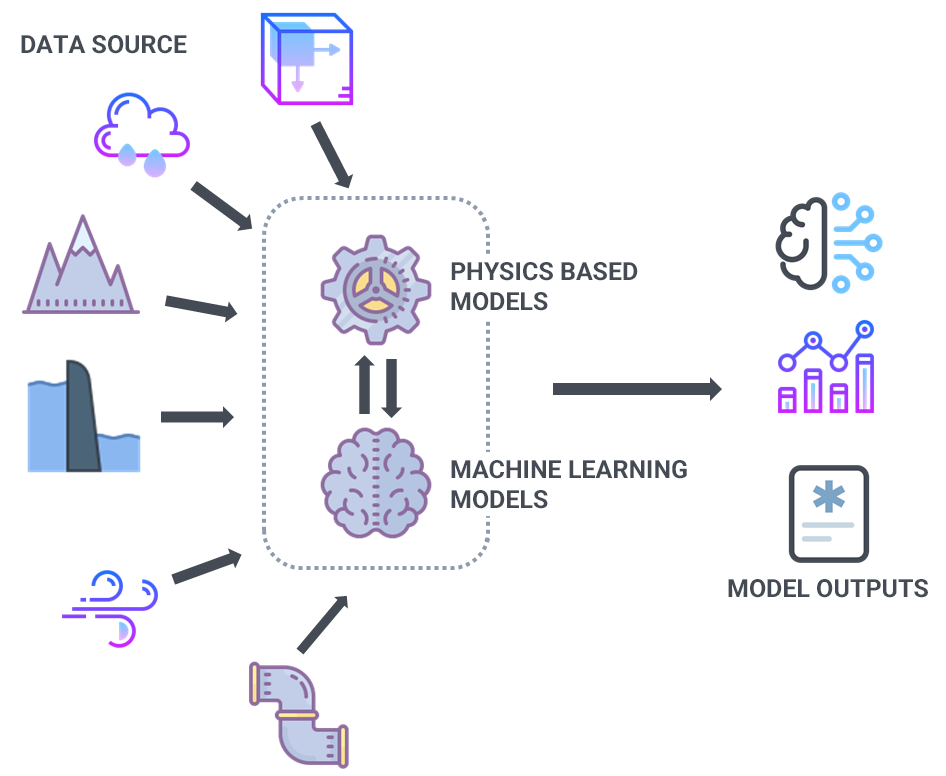
\includegraphics[width=1\textwidth]{graphics/machine-learning-illu}
\par\end{center}

\foilhead{Recall: Differentiable programming}
\begin{itemize}
\item Differential programming is a technique for \textcolor{magenta}{automatically
computing the derivatives} of functions. 
\item This can be done using a variety of techniques, including: 
\begin{itemize}
\item \textbf{Symbolic differentiation}
\item \textbf{Numerical differentiation}
\item \textbf{\textcolor{magenta}{Automatic differentiation}}: This is a
technique that combines symbolic and numerical differentiation to
automatically compute the derivatives of functions. This is the most
powerful technique for differential programming, and it is the most
commonly used technique in scientific machine learning. 
\end{itemize}
\item The mathematical theory of differential programming is based on the
concept of \textcolor{magenta}{gradients}. 
\item Differential programming can be used to solve a variety of problems
in scientific machine learning, including: 
\begin{itemize}
\item Calculating the \textcolor{magenta}{gradients of loss functions} for
machine learning models.
\item Solving \textcolor{magenta}{differential equations.}
\item Performing \textcolor{magenta}{optimization.}
\item Solving \textbf{\textcolor{magenta}{inverse and data assimilation
problems.}}
\end{itemize}
\end{itemize}

\foilhead{Recall: Automatic Differentiation}
\begin{itemize}
\item Automatic differentiation is an umbrella term for a variety of techniques
for efficiently computing accurate derivatives of more or less general
programs. 
\item Many algorithms in machine learning, computer vision, physical simulation,
and other fields require the calculation of gradients and other derivatives. 
\item Practitioners across many fields have built a wide set of \textcolor{magenta}{automatic
differentiation tools}, using different programming languages, computational
primitives, and intermediate compiler representations. 
\item AD can be readily and extensively used and is thus applicable to many
industrial and practical \textcolor{magenta}{Digital Twin} contexts
\cite{Asch2022}.
\end{itemize}

\foilhead{AD for SciML}
\begin{itemize}
\item Recent progress in machine learning (ML) technology has been spectacular.
\item At the heart of these advances is the ability to obtain high-quality
solutions to\textcolor{magenta}{{} non-convex optimization problems}
for functions with billions---or even hundreds of billions---of
parameters.
\item Incredible \textcolor{magenta}{opportunity} for progress in classical
applied mathematics problems.
\end{itemize}

\foilhead{Automatic Differentiation---backprop, autograd, etc.}
\begin{itemize}
\item \textcolor{magenta}{Backprop} is a special case of autodiff.
\item \textcolor{magenta}{Autograd} is a particular autodiff package.
\item In practice, we will pricipally use \textcolor{magenta}{PyTorch}'s
autodiff functions.
\end{itemize}
\begin{rem}
Autodiff is \textcolor{magenta}{NOT} finite differences, nor symbolic
differentiation. Finite differences are too \textcolor{magenta}{expensive}
(one forward pass for each discrete point). They induce huge \textcolor{magenta}{numerical
errors} (truncation/approximation and roundoff) and are very unstable
in the presence of noise.
\end{rem}
~
\begin{rem}
Autodiff is both \textcolor{magenta}{efficient}---linear in the cost
of computing the value---and numerically \textcolor{magenta}{stable}. 
\end{rem}
~
\begin{rem}
The goal of autodiff is not a formula, but a \textcolor{magenta}{procedure}
for computing derivatives.
\end{rem}

\foilhead{Tools for AD}
\begin{itemize}
\item New opportunities that exist because of the widespread, open-source
deployment of effective \textcolor{magenta}{software tools for automatic
differentiation}. 
\item Efficient software frameworks that natively run on \textcolor{magenta}{hardware
accelerators} (GPUs). 
\item These frameworks inspired \textcolor{magenta}{high-quality software}
libraries such as 
\begin{itemize}
\item JAX, 
\item \textcolor{magenta}{PyTorch},
\item TensorFlow. 
\end{itemize}
\item The technology\textquoteright s key feature is: \textbf{the computational
cost of computing derivatives of a target loss function is independent
of the number of parameters;}
\begin{itemize}
\item this trait makes it possible for users to implement \textcolor{magenta}{gradient-based
optimization} algorithms for functions with staggering numbers of
parameters.
\end{itemize}
\end{itemize}

\foilhead{AD Sayings}
\begin{quote}
\textcolor{orange}{``Gradient descent can write code better than you,
I'm sorry.'' }

\textcolor{orange}{``Yes, you should understand backprop.'' }

\textcolor{orange}{``I've been using PyTorch a few months now and
I've never felt better. I have more energy. My skin is clearer. My
eye sight has improved.''}
\end{quote}
\begin{itemize}
\item Andrej Karpathy {[}\textasciitilde 2017{]} (Tesla AI, OpenAI)
\end{itemize}

\foilhead{Why use ML/Neural Networks for SciML?}
\begin{itemize}
\item Excellent, \textcolor{magenta}{open-source} tools and frameworks
\begin{itemize}
\item Autodiff
\item PyTorch
\item many, many others...
\end{itemize}
\item \textcolor{magenta}{Universal approximation property} (UAP for NNs)
\item Curse of \textcolor{magenta}{dimensionality}
\end{itemize}

\foilhead{Recall: what is a NN?}
\begin{itemize}
\item A Neural Network is a \textcolor{magenta}{composition} of nonlinear
functions (see Basic Course)
\[
\mathrm{NN}(x)=W_{3}\sigma_{2}\left(W_{2}\sigma_{1}\left(W_{1}x+b_{1}\right)+b_{2}\right)+b_{3}
\]
 where we can add layers, and to each layer, add neurons.
\item \textcolor{magenta}{Training} a NN: given \textcolor{magenta}{observations}
$y=f(x)$ of some unknown function $f,$ find the values of $W$ that
minimize the \textcolor{magenta}{loss function} expressing the mismatch
between the predictions of $\mathrm{NN}(x)$ and the corresponding
values of $y.$
\begin{itemize}
\item hence the NN is just a \textcolor{magenta}{function approximator}
\end{itemize}
\end{itemize}

\foilhead{Recall: why NNs?}
\begin{itemize}
\item Neural Networks have two important properties:
\begin{itemize}
\item \textcolor{magenta}{Universal Approximation} property, which states
that for a given accuracy $\epsilon,$ one can construct a large NN
such that it can approximate any (reasonable) function $f,$ of arbitrary
complexity, within the tolerance $\epsilon.$
\item Avoidance of the \textcolor{magenta}{Curse of Dimensionality}. If
we were to make a polynomial approximation with $n$ coefficients
in each of $d$ dimensions, then the complexity of this approximator
will exponential in $d.$ However, the \textcolor{magenta}{growth}
of a NN to sufficiently approximate a $d$-dimensional function, only
grows as a \textcolor{magenta}{polynomial} in $d.$
\end{itemize}
\end{itemize}

\foilhead{Recall: Universal Approximation for Functions}
\begin{thm}
[Cybenko 1989]If $\sigma$ is any continuous sigmoidal function,
then finite sums 
\[
G(x)=\sum_{j=1}^{N}\alpha_{j}\sigma\left(y_{j}\cdot x+\theta_{j}\right)
\]
 are dense in $C(I_{d}).$
\end{thm}
%
\vspace{.5\baselineskip}

\vspace{.5\baselineskip}

\begin{thm}
[Pinkus 1999]Let $\mathbf{m}_{i}\in\mathbb{Z}^{d},$ $i=1,\ldots,s,$
and set $m=\max_{i}\left|\mathbf{m}^{i}\right|.$ Suppose that $\sigma\in C^{m}(\mathbb{R}),$
not polynomial. Then the space of \textcolor{red}{single hidden layer}
neural nets, 
\[
\mathcal{M}(\sigma)=\mathrm{span}\left\{ \sigma(\mathbf{w}\cdot\mathbf{x}+b)\colon\mathbf{w}\in\mathbb{R}^{d},\,b\in\mathbb{R}\right\} ,
\]
is dense in $C^{\mathbf{m}^{1},\ldots,\mathbf{m}^{s}}(\mathbb{R}^{d})\doteq\cap_{i=1}^{s}C^{\mathbf{m}^{i}}(\mathbb{R}^{d}).$
\end{thm}
\begin{center}\index{neural networks (NN)!multi layer perceptron (MLP)|ffi}
\def\layersep{2.5cm}
\begin{tikzpicture}[shorten >=1pt,->,draw=black!50, node distance=\layersep, scale=1.4, transform shape]
\tikzstyle{every pin edge}=[<-,shorten <=1pt]
\tikzstyle{neuron}=[circle,fill=black!25,minimum size=17pt,inner sep=0pt]
\tikzstyle{input neuron}=[neuron, fill=green!50];
\tikzstyle{output neuron}=[neuron, fill=red!50];
\tikzstyle{hidden neuron}=[neuron, fill=blue!50];
\tikzstyle{annot} = [text width=4em, text centered]

% Draw the input layer nodes
\foreach \name / \y in {1,...,4}
% This is the same as writing \foreach \name / \y in {1/1,2/2,3/3,4/4}
\node[input neuron, pin=left:Input $x_{\y}$] (I-\name) at (0,-\y) {};

% Draw the hidden layer nodes
\foreach \name / \y in {1,...,5}
\path[yshift=0.5cm]
node[hidden neuron] (H-\name) at (\layersep,-\y cm) {};

% Draw the output layer node
\node[output neuron,pin={[pin edge={->}]right:Output $y$}, right of=H-3] (O) {};

% Connect every node in the input layer with every node in the
% hidden layer.
\foreach \source in {1,...,4}
\foreach \dest in {1,...,5}
\path (I-\source) edge (H-\dest);

% Connect every node in the hidden layer with the output layer
\foreach \source in {1,...,5}
\path (H-\source) edge (O);

% Annotate the layers
\node[annot,above of=H-1, node distance=2cm] (hl) {Hidden layer};
\node[annot,left of=hl] {Input layer};
\node[annot,right of=hl] {Output layer};
\end{tikzpicture}
\end{center}

\foilhead{From ML to SciML...}
\begin{itemize}
\item In \textcolor{magenta}{scientific machine learning}, neural networks
and machine learning are used as the basis to solve problems in CSE
(Computational Science and Engineering)
\item CSE is, in majority, driven by systems of\textcolor{magenta}{{} (P)DEs},
since we are interested in how systems \textcolor{magenta}{evolve/change}.
\begin{itemize}
\item As a consequence, the use of ML for the solution of differential eqations
is an important topic.
\item As we will see, ML can be used in other ways too.
\end{itemize}
\end{itemize}

\foilhead{ML/NN Approaches}
\begin{itemize}
\item Recall the ``question of balance''
\end{itemize}
\begin{center}
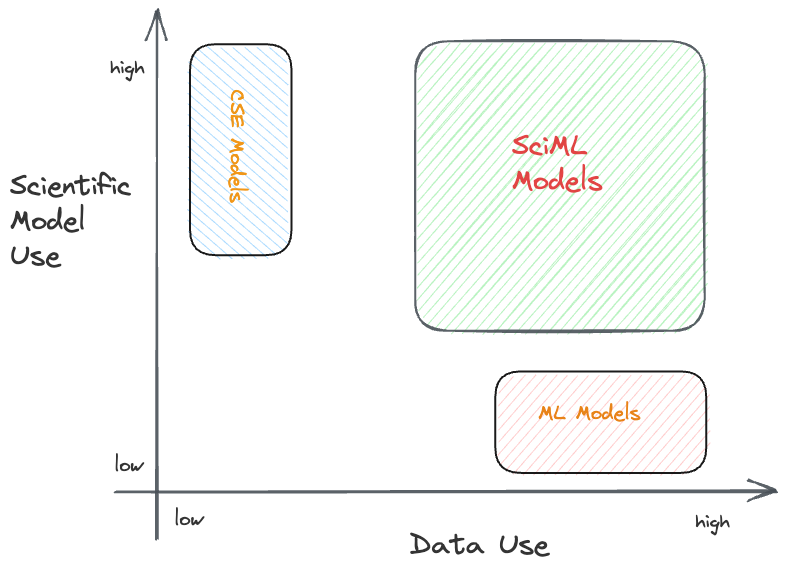
\includegraphics[width=0.8\textwidth]{graphics/data_model_sciml}
\par\end{center}
\begin{itemize}
\item Now, we are going,to decompose the SciML block into classes... (there
are several ways of doing this)
\item 3 major classes of approaches
\begin{itemize}
\item architecture-based
\item loss function 
\item hybrid approaches
\end{itemize}
\item 4 widely-used families of approaches:
\begin{itemize}
\item SUMO - surrogate modeling
\item PCL - physics constrained learning
\item PINN - physics informed neural networks
\item DeepONet/PINO/FNO - neural operators
\end{itemize}
\item Others:
\begin{itemize}
\item Neural ODEs
\item Differentiable physics
\item Koopman theory
\end{itemize}
\item An alternative classification:
\begin{itemize}
\item constrained (including PINN and PCL)
\item encoded (DL-type architectures)
\item operator-based (DeepONet, FNO)
\end{itemize}
\item SUMO then falls into the ``data-driven'' category
\end{itemize}

\foilhead{Forward and Inverse Problems}
\begin{center}
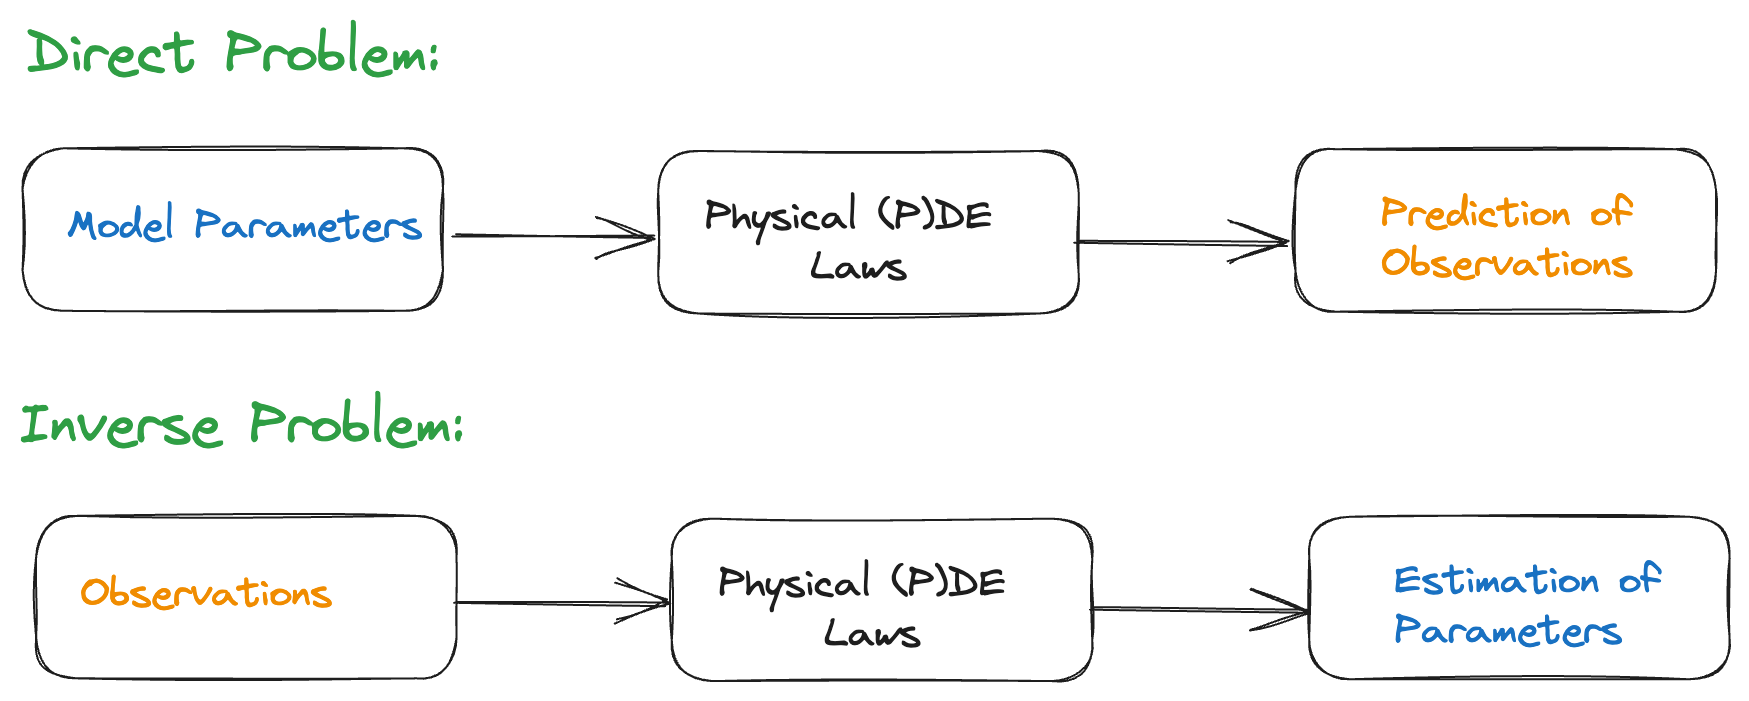
\includegraphics[scale=0.3]{graphics/direct_inverse}
\par\end{center}
\begin{itemize}
\item \textcolor{magenta}{Forward} simulation is a major CSE task: predict
the system's evolution, given some input conditions.
\begin{itemize}
\item Usually we solve a system of diffferential equations with some forcing
and boundary conditions
\item \textbf{Challenges}: 
\begin{itemize}
\item major challenge is the extremely high computational costs of simulating
complex, multi-scale, multi-physics systems.
\item quantifying uncertainty for predictions/forecasts
\end{itemize}
\item SciML is helping to alleviate these issues by allowing the possibility
to learn from previous simulations, providing more powerful computational
shortcuts whilst having less impact on the simulation fidelity
\end{itemize}
\item \textcolor{magenta}{Inverse} problems are tightly related to simulation
and solving them is crucial for many real-world tasks. 
\begin{itemize}
\item Here the goal is to estimate a set of latent, hidden, or unobserved
parameters of a system given a set of real-world observations of the
system.
\item \textbf{Challenges}:
\begin{itemize}
\item Inversion algorithms often require many forward simulations to be
run in order to match the predictions of the physical model to the
set of observations.
\item Given the potentially high computational costs of forward simulation
stated above, this can render many IP applications unfeasible. 
\item Inversion problems generally suffer from ill-posedness. 
\item In such cases, sophisticated regularization schemes are required to
restrict the space of possible latent parameters the inversion algorithm
can explore.
\item Finally, real-world inversion usually suffers from noise/uncertainty.
This is challenging to quantify and will increase the ill-posedness
of the problem.
\item Often a fully probabilistic framework is required to model such processes.
\end{itemize}
\end{itemize}
\end{itemize}

\foilhead{$\;$}

\vfill{}

\begin{center}
{\Large\textbf{\textcolor{blue}{EQUATION DISCOVERY}}}{\Large\par}
\par\end{center}

\vfill{}


\foilhead{Equation Discovery}
\begin{itemize}
\item There are many contexts where we do not fully understand the system
itself.
\item We are unsure how to define the model $\mathcal{F}$---this is a
type of inverse problem.
\item Being able to learn about a system, for example by discovering its
governing equations, is powerful as it can provide a general model
of the system.
\item SciML is aiding this discovery by allowing us to automate the process
and/or learn about complex processes which are hard to intuit 
\end{itemize}

\foilhead{Equation Discovery: theory}
\begin{itemize}
\item Suppose we have a \textcolor{magenta}{dynamic} system
\begin{equation}
\frac{d}{dt}\mathbf{x}{(t)}=\mathbf{f}{(\mathbf{x}{(t)})},
\end{equation}
 where
\begin{itemize}
\item vector $\mathbf{x}{(t)}$ denotes the state of a system at time $t,$
\item the function $\mathbf{f}$ represents the dynamic constraints that
define the equations of motion of the system, such as Newton\textquoteright s
second law. 
\item The dynamics can be generalized to include parameterization, time
dependence, and forcing.
\end{itemize}
\item \textbf{Key observation}: for many systems of interest, the function
$\mathbf{f}$ consists of only a few terms, making it \textcolor{magenta}{sparse}
in the space of possible functions.
\item To determine the function $\mathbf{f}$ from data, 
\begin{itemize}
\item we collect a time history of the state $\mathbf{x}{(t)}$
\item and either measure the derivative $\mathbf{\dot{x}}{(t)}$ or approximate
it numerically from $\mathbf{x}{(t)}$
\item The data are sampled at several times $t_{1},\ldots,t_{m}$ and arranged
into two matrices:
\end{itemize}
\end{itemize}
\[
\mathbf{X}=\left[\begin{array}{c}
\mathbf{x}^{\mathrm{T}}(t_{1})\\
\mathbf{x}^{\mathrm{T}}(t_{2})\\
\vdots\\
\mathbf{x}^{\mathrm{T}}(t_{m})
\end{array}\right]=\overset{\longrightarrow\mathrm{state}\longrightarrow}{\left[\begin{array}{cccc}
x_{1}(t_{1}) & x_{2}(t_{1}) & \cdots & x_{n}(t_{1})\\
x_{1}(t_{2}) & x_{2}(t_{2}) & \cdots & x_{n}(t_{2})\\
\vdots & \vdots & \ddots & \vdots\\
x_{1}(t_{m}) & x_{2}(t_{m}) & \cdots & x_{n}(t_{m})
\end{array}\right]\begin{array}{c}
\\\downarrow\\
\mathrm{t}\\
\downarrow
\end{array}}
\]
and similarly for $\mathbf{\dot{X}}$
\begin{itemize}
\item Next, we construct a library $\Theta(\mathbf{X})$ made up of \textcolor{magenta}{candidate
}nonlinear functions of the columns of $\mathbf{X}$
\begin{itemize}
\item For example, $\Theta(\mathbf{X})$ may consist of constant, polynomial,
and trigonometric terms:
\end{itemize}
\end{itemize}
\[
\mathrm{\Theta}{(\mathbf{X})}=\left[\begin{array}{lccccccc}
\overset{\vert}{\underset{\vert}{1}} & \overset{\vert}{\underset{\vert}{\mathbf{X}}} & \overset{\vert}{\underset{\vert}{\mathbf{X}^{P_{2}}}} & \overset{\vert}{\underset{\vert}{\mathbf{X}^{P_{3}}}} & \cdots & \overset{\vert}{\underset{\vert}{\text{sin}{(\mathbf{X})}}} & \overset{\vert}{\underset{\vert}{\text{cos}{(\mathbf{X})}}} & \cdots\end{array}\right].
\]

\begin{itemize}
\item Each column of $\Theta(\mathbf{X})$ represents a candidate function
for the right-hand side of Eq. 1. 
\item There is tremendous freedom in choosing the entries in this matrix
of nonlinearities, because we believe that only a few of these nonlinearities
are active in each row of $\mathbf{f}$ 
\item We set up a\textcolor{magenta}{{} sparse regression} problem to determine
the sparse vectors of coefficients 
\[
\mathrm{\Xi}=\left[\begin{array}{cccc}
{\boldsymbol{\xi}}_{1} & {\boldsymbol{\xi}}_{2} & \cdots & {\boldsymbol{\xi}}_{n}\end{array}\right]
\]
that determine which nonlinearities are active,
\[
\mathbf{\dot{X}}=\mathrm{\Theta}{(\mathbf{X})}\mathrm{\Xi}
\]
\item Each column $\boldsymbol{\xi}_{k}$ of $\mathrm{\Xi}$ is a sparse
vector of coefficients determining which terms are active in the right-hand
side for one of the row equations 
\[
\mathbf{\dot{x}}_{k}=\mathbf{f}_{k}(\mathbf{x})
\]
in Eq. 1. 
\item Once $\mathrm{\Xi}$ has been determined, a model of each row of the
governing equations may be constructed as follows,
\[
\mathbf{\dot{x}}_{k}=\mathbf{f}_{k}(\mathbf{x})=\Theta(\mathbf{x}^{\mathrm{T}})\boldsymbol{\xi}_{k}
\]
\item Note that $\Theta(\mathbf{x}^{\mathrm{T}})$ is a vector of symbolic
functions of elements of $\mathbf{x},$ as opposed to $\mathrm{\Theta}(\mathbf{X}),$
which is a data matrix. 
\item Thus,
\[
\mathbf{\dot{x}}_{k}=\mathbf{f}_{k}(\mathbf{x})=\mathrm{\Xi}^{\mathrm{T}}\left(\Theta(\mathbf{x}^{\mathrm{T}})\right)^{\mathrm{T}}
\]
\end{itemize}

\rotatefoilhead{SINDy Scheme}

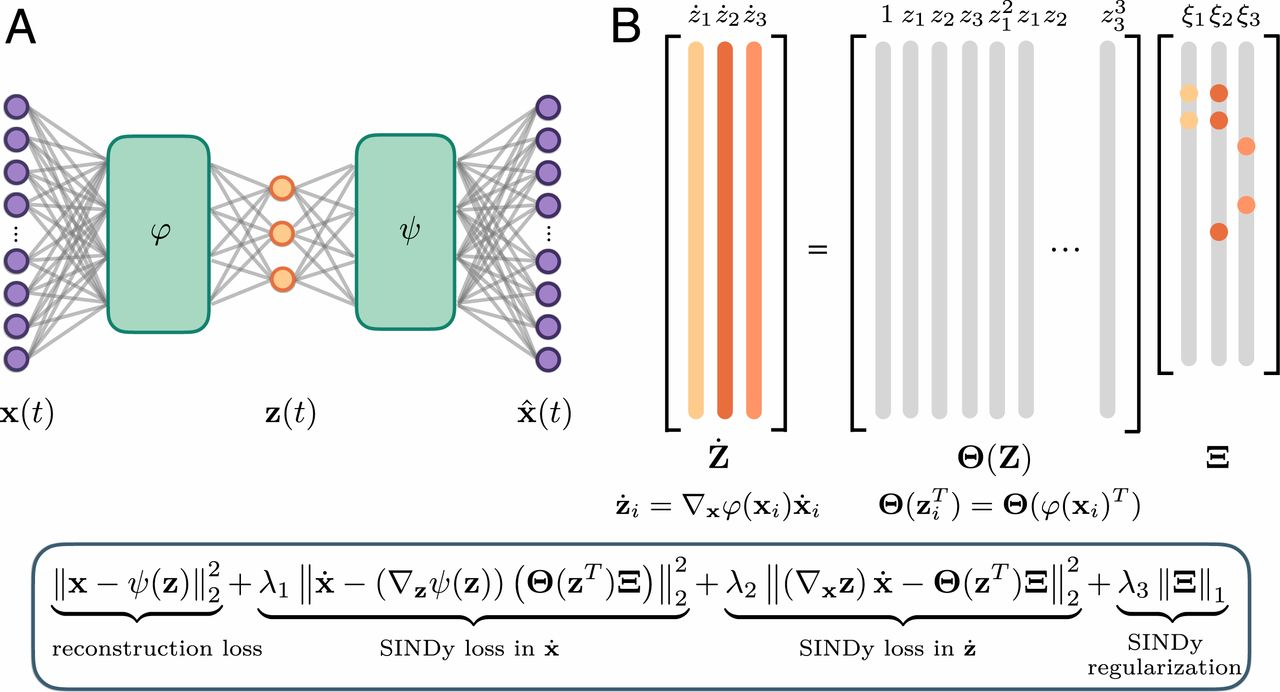
\includegraphics[width=0.9\textwidth]{graphics/SINDYfig01.jpeg}

\rotatefoilhead[-0.5in]{SINDy Application}

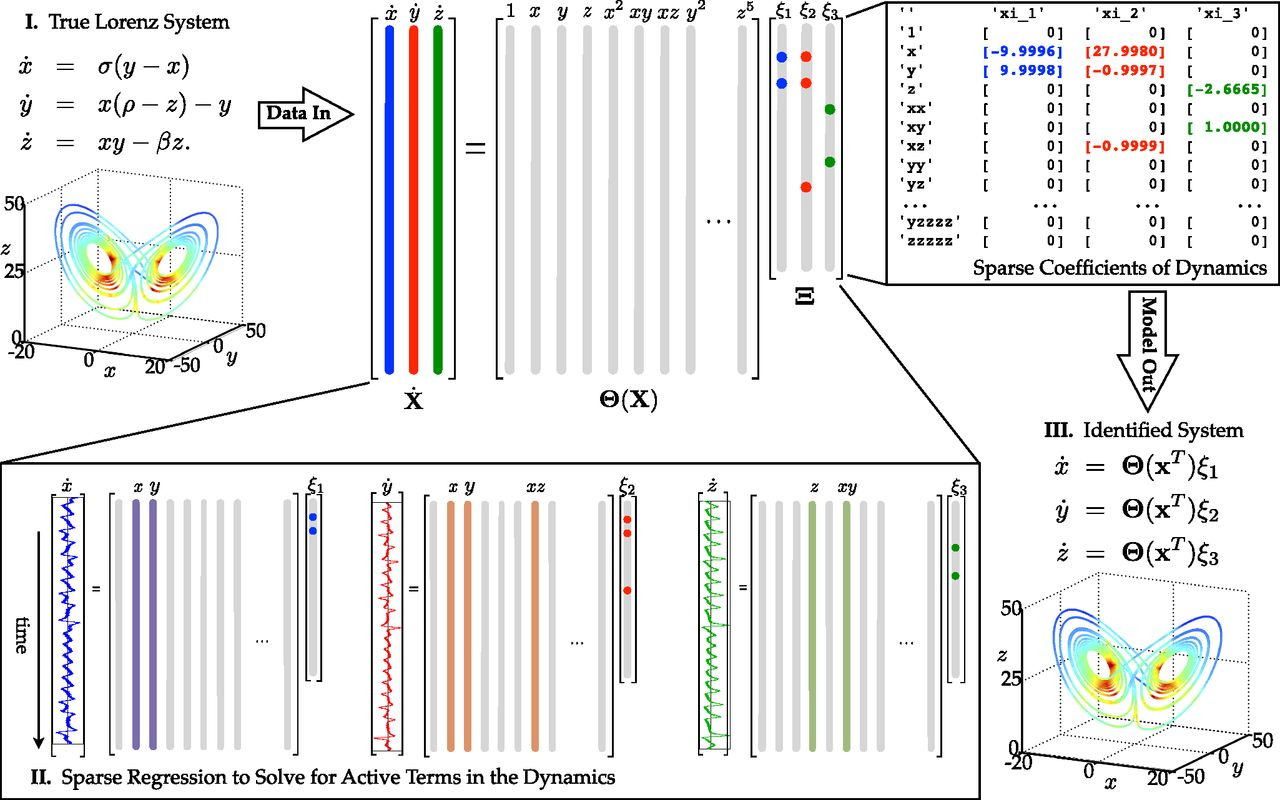
\includegraphics[width=0.85\textwidth]{graphics/SINDyLorenzfig02.jpeg}

\foilhead{Equation Discovery: SINDy references}
\begin{itemize}
\item Code: \\
\textcolor{blue}{\url{https://faculty.washington.edu/kutz/page26/}}
\item Paper: \\
{\small\textcolor{blue}{\url{https://www.pnas.org/doi/10.1073/pnas.1906995116}}}{\small\par}
\end{itemize}

\foilhead{$\;$}

\vfill{}

\begin{center}
{\Large\textbf{\textcolor{blue}{ARCHITECTURE BASED METHODS}}}{\Large\par}
\par\end{center}

\vfill{}


\foilhead{Architecture-based SciML}
\begin{itemize}
\item \textbf{Idea}: change the \textcolor{magenta}{architecture} used in
the ML algorithm so that it incorporates \textcolor{magenta}{scientific
constraints}.
\begin{itemize}
\item we open up the black box's design and change parts of it so that it
\textcolor{magenta}{obeys} these constraints. 
\item Incorporating scientific principles in this way can restrict the range
of models the algorithm can learn, and result in more generalisable
and \textcolor{magenta}{interpretable} models. 
\item From a machine learning perspective, we are introducing a strong \textcolor{magenta}{inductive
bias} into the model.
\item These aspects will be more fully discussed in later lectures on \textcolor{blue}{Bias
and Ethics of ML}.
\end{itemize}
\item Approaches
\begin{itemize}
\item encode certain physical \textcolor{magenta}{variables}, for example
using an LSTM for intermediate variables 
\item encode \textcolor{magenta}{symmetries}, such as translational and
rotational invariance---this can be easily achieved with convolutional
neural networks (CNNs)
\item use \textcolor{magenta}{Koopman} theory {[}Brunton, Kutz{]}
\item use physically constrained \textcolor{magenta}{Gaussian} processes
\end{itemize}
\end{itemize}

\foilhead{$\;$}

\vfill{}

\begin{center}
{\Large\textbf{\textcolor{blue}{SURROGATE MODELING}}}{\Large\par}
\par\end{center}

\vfill{}


\foilhead{Surrogate Modelling - SUMO}
\begin{itemize}
\item Surrogate modeling is a technique used to approximate a complex and
\textcolor{magenta}{expensive-to-evaluate} function with a simpler
and \textcolor{magenta}{cheaper-to-evaluate} function. 
\item The surrogate model, also known as a metamodel or emulator, is \textcolor{magenta}{trained}
on a set of input-output data from the complex function. 
\item Once trained, the surrogate model can be used to \textcolor{magenta}{predict}
the output of the complex function for any input value, without having
to evaluate the complex function directly.
\end{itemize}

\foilhead{Surrogate Modelling - formulation }
\begin{itemize}
\item The mathematical presentation of surrogate modeling depends on the
specific type of surrogate model being used. 
\item However, there is a general framework that can be applied to most
surrogate models.
\begin{itemize}
\item Let $f(x)$ be the \textcolor{magenta}{complex function} that we want
to approximate, and let $s(x)$ be the \textcolor{magenta}{surrogate
model}. 
\end{itemize}
\item The \textcolor{magenta}{goal of surrogate modeling} is to find a surrogate
model$s(x)$that is as close to the complex function $f(x$) as possible,
given a limited amount of training data.
\item One way to measure the similarity between the complex function and
the surrogate model is to use the \textcolor{magenta}{mean squared
error} (MSE):
\[
\mathrm{MSE}=\frac{1}{N}\sum_{i=1}^{N}(f(x_{i})-s(x_{i}))^{2}
\]
where $N$ is the number of training data points, and $x_{i}$ and
$f(x_{i})$ are the $i$-th input-output pair in the training dataset.
\item The surrogate model can be trained using a \textcolor{magenta}{variety
of machine learning algorithms}, such as kriging, radial basis functions
(RBFs), support vector machines (SVMs), and artificial neural networks
(ANNs).
\end{itemize}

\foilhead{Surrogate Modelling - formulation II}
\begin{itemize}
\item Given a set of \textcolor{magenta}{training} data points 
\[
{(x_{1},y_{1}),(x_{2},y_{2}),...,(x_{n},y_{n})},
\]
where $x_{i}$ is the input vector and $y_{i}$ is the output value,
the goal of surrogate modeling is to construct a function $\hat{y}(x)$
that approximates the true function $y(x)$ as accurately as possible.
\item The most common approach to surrogate modeling is to use a \textcolor{magenta}{statistical
model}, such as a polynomial response surface, kriging, or support
vector machine. These models can be trained on the training data points
to learn the relationship between the inputs and outputs.
\item Once the surrogate model is trained, it can be used to \textcolor{magenta}{predict
}the output value for any input value x as follows:
\end{itemize}
\[
\hat{y}(x)=\text{Model}(x)
\]

where $\textrm{Model}(x)$ is the output of the surrogate model.

\foilhead{Surrogate Modelling - examples }

Surrogate modeling is used in a wide variety of applications, including:
\begin{itemize}
\item Engineering design: Surrogate models can be used to accelerate the
design process by providing cheaper and faster predictions of the
performance of different design alternatives.
\item Scientific computing: Surrogate models can be used to reduce the computational
cost of simulating complex physical systems.
\item Financial modeling: Surrogate models can be used to predict the risk
and return of financial investments.
\item Machine learning: Surrogate models can be used to interpret the predictions
of complex machine learning models.
\end{itemize}
Here are some specific examples of surrogate modeling in use:
\begin{itemize}
\item Aerospace engineering: Surrogate models are used to design aircraft
wings, engines, and other components.
\item Automotive engineering: Surrogate models are used to design car engines,
suspensions, and other components.
\item Chemical engineering: Surrogate models are used to design chemical
reactors, pipelines, and other equipment.
\item Oil and gas exploration: Surrogate models are used to predict the
flow of oil and gas through reservoirs.
\item Pharmaceutical development: Surrogate models are used to predict the
properties of drugs and to design clinical trials.
\end{itemize}
\textbf{Conclusion}

Surrogate modeling is a\textcolor{magenta}{{} powerful technique }for
approximating complex and expensive-to-evaluate functions. It is used
in a wide variety of applications, including engineering design, scientific
computing, financial modeling, and machine learning.

\foilhead{Surrogate Modelling - in practice}
\begin{defn}
\textcolor{magenta}{Surrogate models}, also known as response surfaces,
black-box models, metamodels, or emulators, are simplified approximations
of more complex, higher order models. These models are used to map
input-data to output-data, when the actual relationship between the
two is unknown or computationally too expensive to evaluate.
\end{defn}
\begin{center}
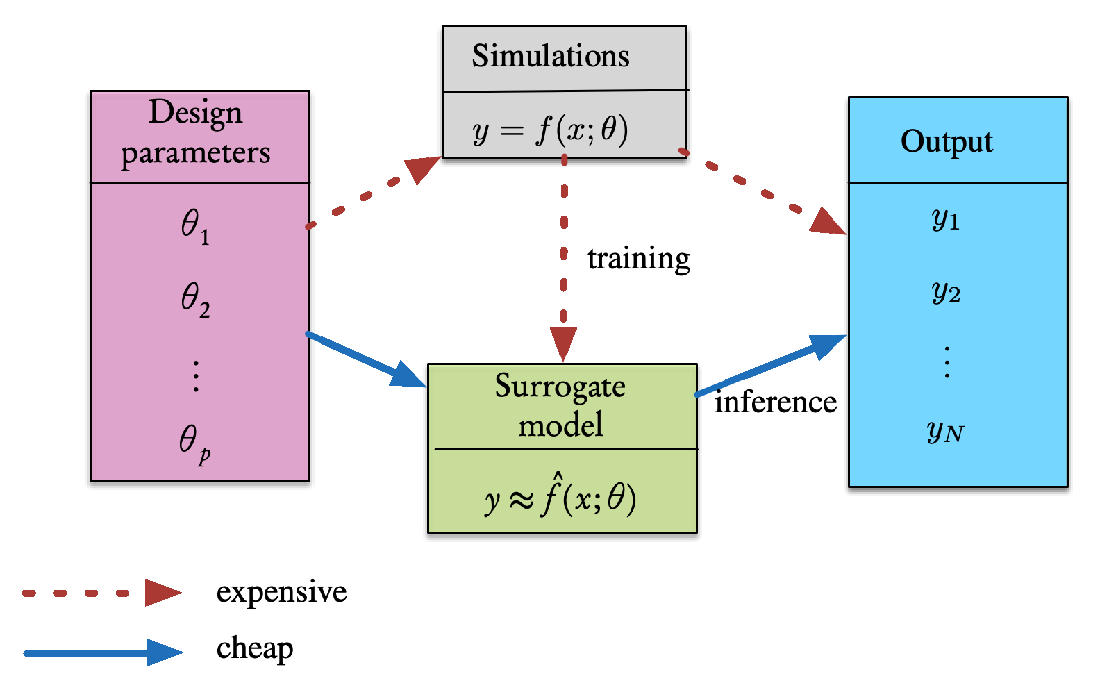
\includegraphics[scale=0.9]{graphics/SUMO}
\par\end{center}
\begin{itemize}
\item \textbf{Idea}: a ML-trained model can \textcolor{magenta}{subsitute}
all or part of a system of (P)DEs
\begin{itemize}
\item learn the complete, unknown input-output relation (but no physics
constraints)
\item learn some sub-parametrization that is too complicated to capture
by classical methods
\end{itemize}
\end{itemize}
The surrogate modeling \textcolor{magenta}{process}, as depicted in
the Figure, consists of \textcolor{magenta}{five stages}: 
\begin{enumerate}
\item Choice of the \textcolor{magenta}{design parameters}. 
\item Generation of input-output pairs of \textcolor{magenta}{data for training},
by simulations of the physics-based model, or from experiments with
varying parameter values. This is the most \textcolor{magenta}{expensive}
step. 
\item Choice of the \textcolor{magenta}{surrogate} model, based on a suitable
supervised machine learning method. 
\item \textcolor{magenta}{Training} of the machine learning model, using
the training data. This can be an expensive step, but is usually only
performed once. 
\item Finally, use of the trained surrogate model to perform computationally
cheap \textcolor{magenta}{inference} for new values of the design
parameters, thus permitting 
\begin{enumerate}
\item an exhaustive search of the parameter space, 
\item an optimal parameter design, and/or 
\item a quantification of design uncertainties. 
\end{enumerate}
\end{enumerate}
\begin{itemize}
\item \textbf{Questions}: 
\begin{itemize}
\item But, can such a surrogate faithfully \textcolor{magenta}{capture}
the complex, nonlinear relationships between input and output? 
\item And, if so, \textcolor{magenta}{how} can the surrogate do this? 
\end{itemize}
\item These two very important questions are fundamental for any underlying
system or process that we would like to study using surrogate modeling. 
\begin{itemize}
\item The answer to the first question is: ``\textcolor{magenta}{Yes},
in theory,'' thanks to the universal approximation property of very
simple machine learning models---fully-connected, feed-forward neural
networks (FCNN) {[}\textcolor{blue}{Cybenko, Pinkus}{]}. 
\item And the answer to the second question is: ``\textcolor{magenta}{Yes},
in practice,'' with the aid of a large variety of supervised learning
techniques, of which FCNNs are just one special case.
\end{itemize}
\end{itemize}

\foilhead{Tecniques for SUMO}
\begin{itemize}
\item Both \textcolor{magenta}{supervised} and \textcolor{magenta}{unsupervised}\footnote{Adversarial and self-supervised are also possible, but far more complicated
to implement.} learning techniques can be used for SUMO.
\item Four of these techniques are recommended, since they are robust and
perform well:
\begin{itemize}
\item \textcolor{magenta}{random forests }and \textcolor{magenta}{multi-layer
perceptrons} (FCNN) in the case of regression, and 
\item support vector machines (\textcolor{magenta}{SVM}) and \textcolor{magenta}{$k$-means}
clustering in the case of classification.
\end{itemize}
\item There is no single, perfect, \textcolor{magenta}{globally} applicable
method that will always do the best job. 
\item Usually, one should try a few, and then settle for the one or two
that are the simplest, but provide \textcolor{magenta}{adequate} precision
and especially robustness in the face of the inherent uncertainties
in the underlying processes---see also the \textcolor{blue}{Ethics
and Bias Lectures}.
\end{itemize}

\foilhead{SUMO Principles}
\begin{itemize}
\item The principle behind the SUMO approach is the following: 
\begin{itemize}
\item if a multiscale, multiphysics relationship between design parameters
and output performance can be \textcolor{magenta}{learned} from data,
then we can forgo---at least to some extent---the underlying ODE,
PDE and population dynamics models, as well as time-consuming, expensive
physical/clinical experiments and trials. 
\item Moreover, once this relationship has been learned, its use---the
so-called \textcolor{magenta}{inference} phase---is very inexpensive
and one can then envisage the solution of optimization and uncertainty
quantification problems
\item We are in fact, constructing a \textcolor{magenta}{digital twin} {[}Asch2022{]}.
\end{itemize}
\item The approach proposed here is \textcolor{magenta}{not} to seek a complex
machine learning model, but to favor \textcolor{magenta}{simpler}
models that are easier to interpret, trust and deploy---see \textcolor{blue}{Ethics
and Bias Lecture}. 
\item These \textcolor{blue}{low-complexity} models will not suffer from
brittleness and will preserve a good bias-variance trade-off. They
will also have more favorable interpretabilty, ethics and bias properties.
\end{itemize}

\foilhead{SUMO - Training Data}
\begin{itemize}
\item To learn a data-driven model, we need\textcolor{magenta}{{} training
data.} 
\item This data is obtained from experimental \textcolor{magenta}{observations},
or model-based \textcolor{magenta}{simulations}, or some combination
of the two. 
\begin{itemize}
\item Here we will often, if possible, use model-based simulations, calculated
for example by a SIR model.
\end{itemize}
\item For any supervised machine learning method, we first need to carefully
select and define \textcolor{magenta}{response variables}---or functions---that
is an unknown function of the input parameters.
\item When defining the output parameters for the machine learning, extreme
care needs to be taken to extract \textcolor{magenta}{reliable} information
describing \textcolor{magenta}{adequately} the phenomenon that we
seek to explore, analyze and forecast
\item Often, sampling techniques must be used to ensure a \textcolor{magenta}{space-filling}
parameter range with good projection properties. 
\item The \textcolor{magenta}{LHS} method is a generalization to higher
dimensions of the \textcolor{magenta}{Latin square }which is an $n\times n$
array filled with $n$ different symbols, each occurring exactly once
in each row and exactly once in each column.
\begin{itemize}
\item Assuming a three dimensional parameter space and $n_{s}$ the number
of samples of each parameter, then each sample is the only one in
each axis-aligned hyperplane containing it. 
\item On the other hand, building an LHS design with the best maximin criterion
on all projections provides a space filling design in the whole space
and on projections. 
\end{itemize}
\item Hence, we obtain a training set that is \textcolor{magenta}{well-balanced},
containing a wide range of behaviors, which in turn will ensure the
best possible training for the machine learning models and then, good
predictions.
\end{itemize}

\foilhead{SUMO - EDA}
\begin{itemize}
\item In order to identify useful preliminary information about the data
and investigate the relationships between the features and the response
variables, an \textcolor{magenta}{exploratory data analysis}---see
\textcolor{blue}{Basic Course Lectures}---should always be performed,
\emph{before} attempting any surrogate modeling.
\item This study can help to detect the \textcolor{magenta}{interactions}
among different variables indiffering contexts, helping us to understand
the importance of their effect on the desired performance of the system.
\item The follwong \textcolor{magenta}{techniques of EDA} should, initially,
be applied (many more are psssible):
\begin{itemize}
\item Summary statistics.
\item Scatter plots.
\item Correlation and partial correlation tables that ensure the non-existence
of \textcolor{magenta}{nuisance} information in the database due to
a confounding variable.
\end{itemize}
\end{itemize}

\foilhead{SUMO - Concrete Workflow Example}

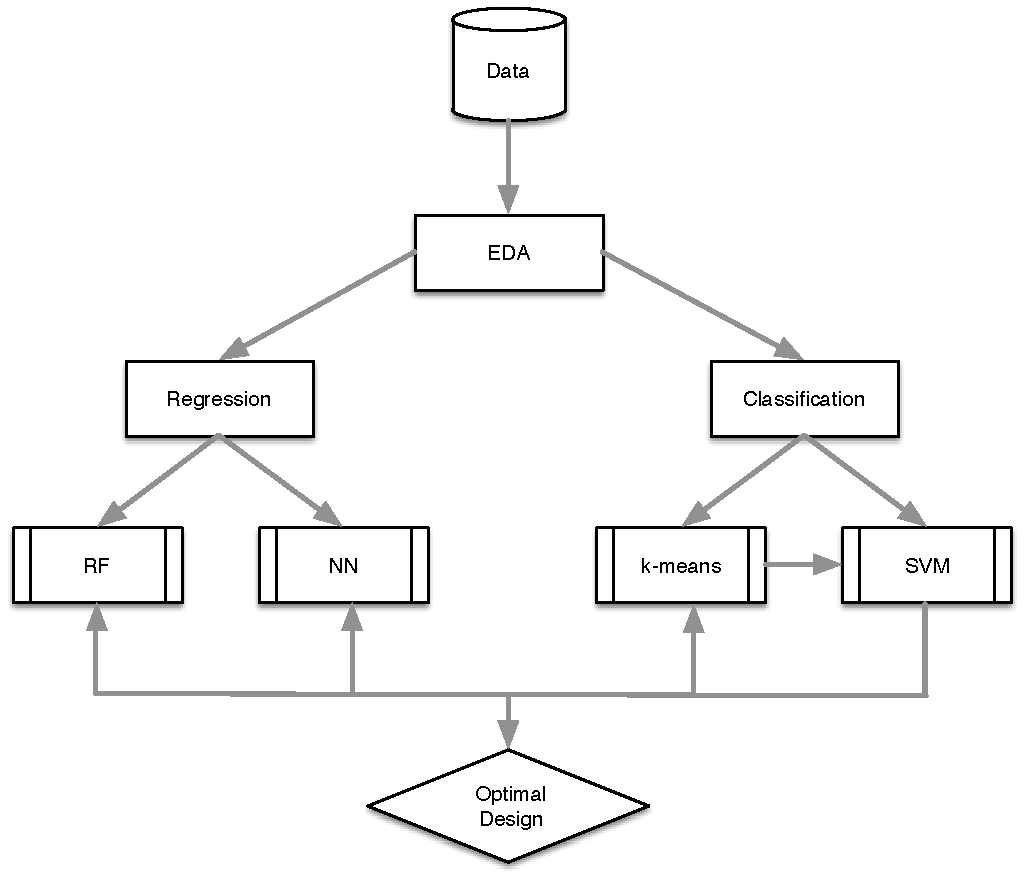
\includegraphics[width=1\textwidth]{graphics/workflow}
\begin{itemize}
\item The approach described above, proposes a \textcolor{magenta}{universal
workflow} for data analysis and surrogate modeling in the light of
optimal design choices. 
\item This workflow, as illustrated in the Figure, can be applied to almost
\textcolor{magenta}{\emph{any}} design/optimization problem.
\begin{itemize}
\item It suffices to replace our data by the reader's data, 
\item our underlying model by the reader's model, 
\item and then simply follow the steps of the workflow.
\end{itemize}
\item Once the data is collected, \textcolor{magenta}{exploratory data analysis}
(EDA) is essential for:
\begin{enumerate}
\item Familiarization with the data and choice of response variables. 
\item Elimination of any unusual, or erroneous data points. 
\item Preliminary identification of the most influential features, or parameters,
and the relations---or lack of relations---between the features
themselves, and between the features and the response variables. 
\item Reduction of the complexity by identification of co-linear variables. 
\end{enumerate}
\item The next steps are \textcolor{magenta}{regression }\textcolor{magenta}{\emph{and}}\textcolor{magenta}{{}
classification.} 
\item Note that classification, especially \textcolor{magenta}{unsupervised},
can be considered as being a part of \textcolor{magenta}{EDA}, since
it can help us in determining response variables.
\item In our proposed workflow, we have purposefully selected \textcolor{magenta}{simple}
approaches because of their 
\begin{itemize}
\item broad applicability, 
\item ease of computation and
\item facility of interpretation---no black boxes here. 
\end{itemize}
\item We highly recommend, for \textcolor{magenta}{regression}:
\begin{enumerate}
\item \textcolor{magenta}{Random forests}, because of their established
robustness and their capacity to rank explanatory variables by their
importance. 
\item \textcolor{magenta}{Neural networks}, of FCNN type, for their extreme
versatility and their universal approximation properties. 
\end{enumerate}
\item We highly recommend, for \textcolor{magenta}{classification}:
\begin{enumerate}
\item \textcolor{magenta}{$k$-means} for initial unsupervised clustering
and identification of groups of properties. 
\item \textcolor{magenta}{SVM }for refined, supervised clustering that provides
a surrogate model. 
\end{enumerate}
\item In the final step, which of course will be context-dependent, we can
exploit all the surrogate models found above for optimal design and
process planning.
\item Once we have a surrogate model, or several surrogate models, at our
disposition, we can address a number of \textcolor{magenta}{outer-loop}
problems {[}Asch2022{]}, such as:
\begin{enumerate}
\item \textcolor{magenta}{Optimization} problems, where we seek to maximize,
or minimize some critical response variables. 
\item \textcolor{magenta}{Uncertainty quantification} problems, where we
seek some kind of confidence interval around the parameter values,
given an estimation of the inherent material or process variabilities. 
\item \textcolor{magenta}{Bayesian optimization} problems, that combine
the above two. 
\end{enumerate}
\item All of these require a large number of simulations, or large volume
of experimental data, that can now be completely replaced by the \textcolor{magenta}{surrogate
model}. 
\begin{itemize}
\item Recall that the evaluation of a surrogate model, whose training has
already been done in an offline computation, can be done in \textcolor{magenta}{quasi-real
time}.
\end{itemize}
\item For the surrogate models themselves, \textcolor{magenta}{other ML
techniques} can be envisaged that could provide further insight and
better predictive power. Among these, we can mention:
\begin{itemize}
\item \textcolor{magenta}{SVM regression} that is well-adapted to highly
nonlinear relationships. 
\item \textcolor{magenta}{Functional data analysis} (FDA) that is particularly
well-suited to time series data. 
\item Further exploration of more sophisticated \textcolor{magenta}{neural
network} architectures. This is particularly indicated in the presence
of multi-physics, or multi-modal data.
\end{itemize}
\item The \textcolor{magenta}{key findings }of the approach presented here
can be summarized as follows. 
\begin{itemize}
\item Firstly, \textcolor{magenta}{exploratory data analysis}, including
correlations, partial correlations and unsupervised classification
by $k$-means, leads to the judicious choice of a few design parameters,
and response variables.
\item Then, supervised classification and regression methods, used together
in \textcolor{magenta}{synergy}, reveal the optimal parameter choices
and propose hitherto unforeseen operating regimes.
\item We can identify the most \textcolor{magenta}{influential} design parameters
and we can characterize the ranges of these parameters and identify
optimal clusterings of these.
\end{itemize}
\end{itemize}

\foilhead{$\;$}

\vfill{}

\begin{center}
{\Large\textbf{\textcolor{blue}{PHYSICS CONSTRAINED LEARNING}}}{\Large\par}
\par\end{center}

\vfill{}


\foilhead{Physics Constrained Learning - PCL}

- \textbf{Idea}: use a NN as part of the (P)DE
\begin{itemize}
\item Given a physical relation
\begin{equation}
F(u;\boldsymbol{\theta})=0\label{eq:PDE}
\end{equation}
represented by an IBVP, or other functional relationship, with
\begin{itemize}
\item $u$ the physical quantity
\item $\boldsymbol{\theta}$ the (material/medium) properties/parameters
\end{itemize}
\item \textcolor{magenta}{Inverse Problem} is defined as: 
\begin{itemize}
\item \textbf{Given} \textcolor{magenta}{observations}/measurements of $u$
at the locations $\mathbf{x}=\left\{ x_{i}\right\} $
\[
\mathbf{u}^{\mathrm{obs}}=\left\{ u(x_{i})\right\} _{i\in\mathcal{I}}
\]
\item \textbf{Estimate} the \textcolor{magenta}{parameters} $\boldsymbol{\theta}$
by minimizing a loss/objective/cost function
\[
L(\boldsymbol{\theta})=\left\Vert u(\mathbf{x})-\mathbf{u}^{\mathrm{obs}}\right\Vert _{2}^{2}
\]
subject to (\ref{eq:PDE}).
\end{itemize}
\end{itemize}

\foilhead{PCL - use of a NN}
\begin{itemize}
\item If $\boldsymbol{\theta}=\boldsymbol{\theta}(x),$ model it by a \textcolor{magenta}{NN}
\[
\boldsymbol{\theta}(x)\approx\mathrm{NN}(x)
\]
\item Express the numerical scheme, such as RK, finite differences, finite,
elements, etc., for approximating the (P)DE (\ref{eq:PDE}) as a \textcolor{magenta}{computational
graph} $G(\boldsymbol{\theta}).$
\item Use \textcolor{magenta}{reverse-mode AD} (aka. backpropagation) to
compute the \textcolor{magenta}{gradient of $L$ }with respect to
$\boldsymbol{\theta}$ and the NN coefficients (weights and biases).
\item \textcolor{magenta}{Minimize} by a suitable gradient algorithm
\begin{itemize}
\item Adam, SGD (1st order)
\item L-BFGS (quasi-Newton)
\item trust-region (2nd order)
\end{itemize}
\end{itemize}

\foilhead{PCL - Recall: use of AD}
\begin{itemize}
\item Optimization problem: $\min_{\theta}L(u)$ subject to $F(\theta,u)=0.$
\item Suppose we have a \textcolor{magenta}{computational graph }for $u=G(\theta).$
\item Then $\tilde{L}(\theta)=L\left(G(\theta)\right)$ and by the IFT we
can compute the \textcolor{magenta}{gradient with respect to $\theta,$}
\begin{itemize}
\item first of $F,$
\[
\frac{\partial F}{\partial\theta}+\frac{\partial F}{\partial u}\frac{\partial G}{\partial\theta}=0,\quad\Rightarrow\quad\frac{\partial G}{\partial\theta}=-\left[\frac{\partial F}{\partial u}\right]^{-1}\frac{\partial F}{\partial\theta}
\]
\item then of $\tilde{L},$ by the chain rule,
\[
\frac{\partial\tilde{L}}{\partial\theta}=\frac{\partial L}{\partial u}\frac{\partial G}{\partial\theta}=-\frac{\partial L}{\partial u}\left[\frac{\partial F}{\partial u}\right]^{-1}\frac{\partial F}{\partial\theta}
\]
\end{itemize}
\item The first derivative is obtained directly from the loss function,
the second and third by reverse-mode AD
\end{itemize}

\foilhead{PCL - applications}
\begin{itemize}
\item PCL has been successfully applied to numerous academic and real-life
problems.
\begin{itemize}
\item Geomechanics, solid mechanics, fluid dynamics, seismic inversion 
\item General approach to inverse modeling: ADCME \url{https://kailaix.github.io/ADCME.jl/latest/ }
{[}Xu, Darve{]}
\end{itemize}
\end{itemize}

\rotatefoilhead[-0.5in]{PCL - applications to stiff (P)DEs}

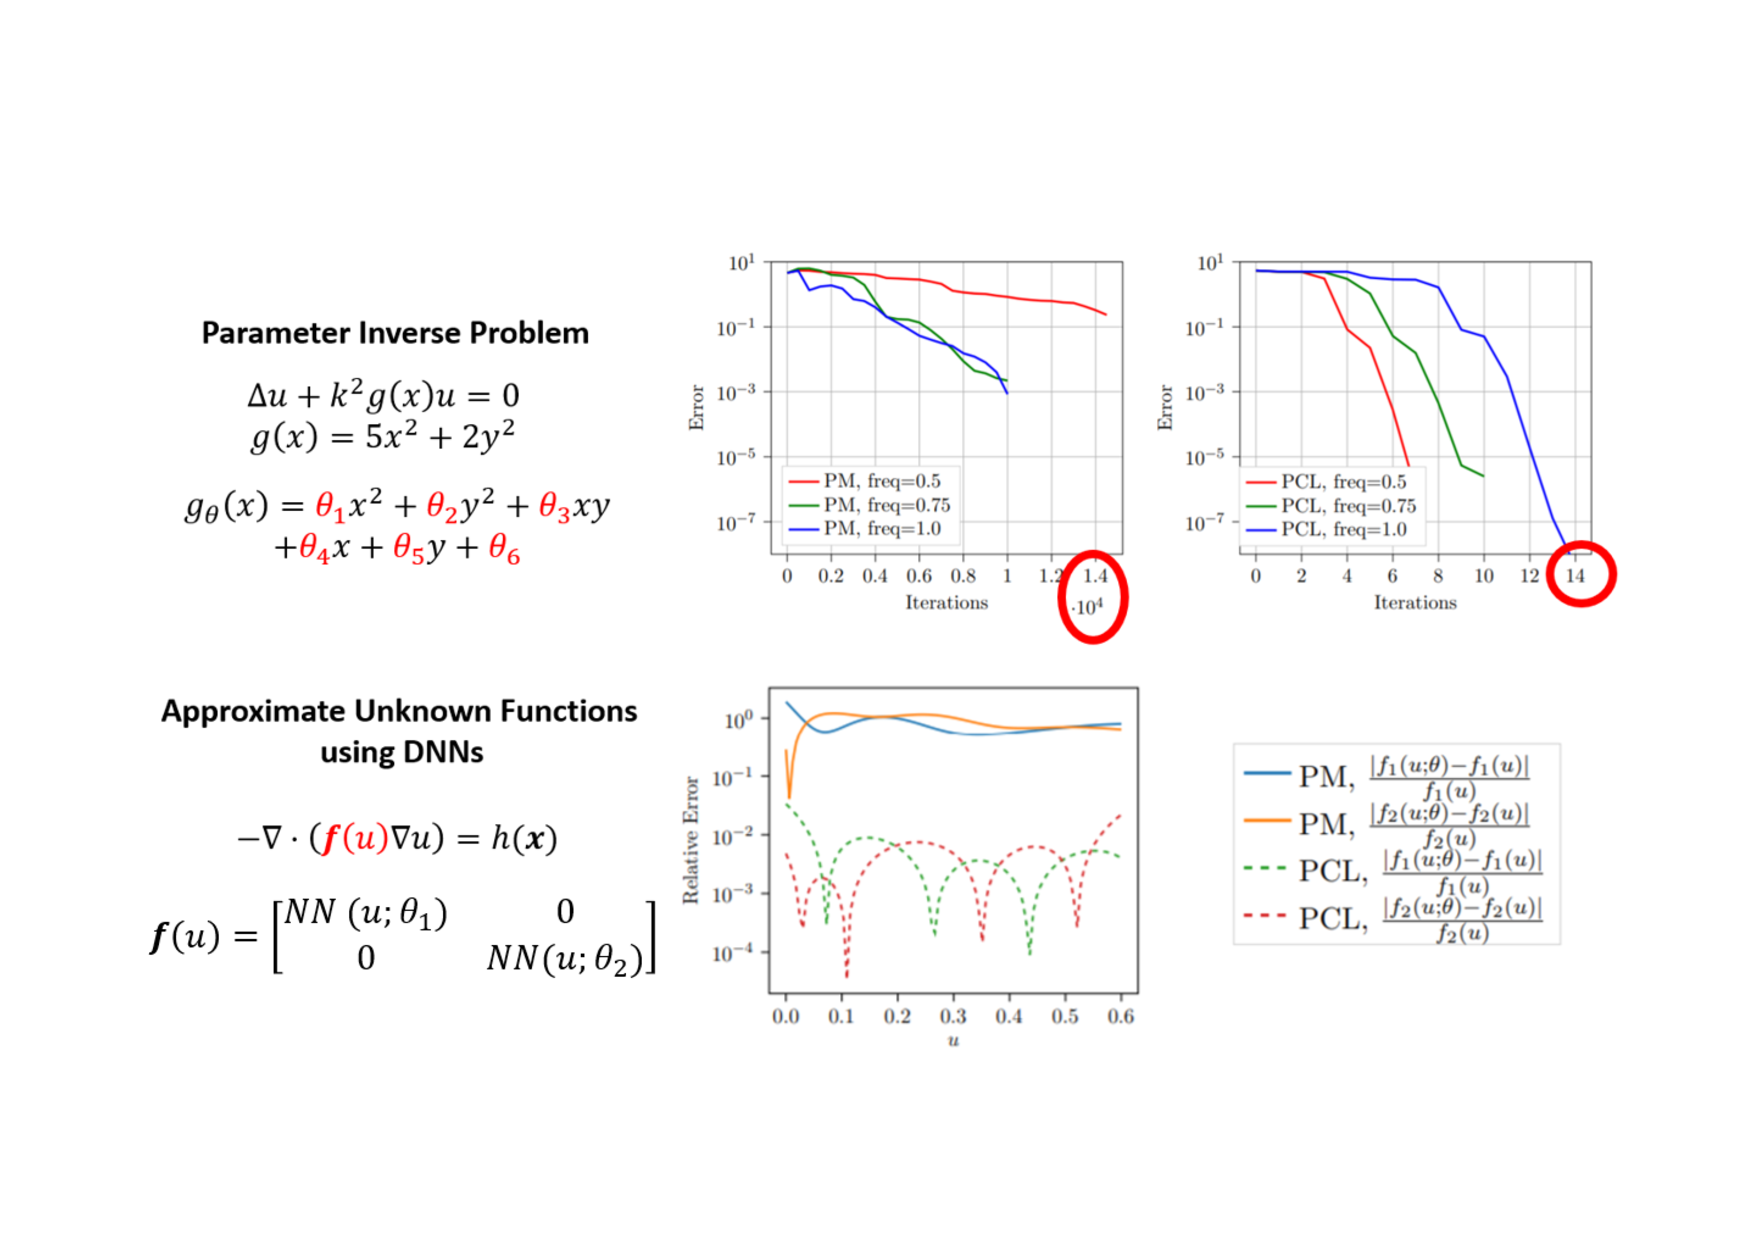
\includegraphics[width=0.9\textwidth]{graphics/PCL_app_Xu}

PM = Penalty Method --- {[}Xu, Darve{]}

\foilhead{$\;$}

\vfill{}

\begin{center}
{\Large\textbf{\textcolor{blue}{PHYSICS INSPIRED LEARNING}}}{\Large\par}
\par\end{center}

\vfill{}


\foilhead{Physics Inspired Neural Networks - PINN background}

- \textbf{Idea}: put the (P)DE into the ML algorithm, via the cost
function (among others)
\begin{itemize}
\item Please review the \textcolor{blue}{Optimization Lecture} for
\begin{itemize}
\item unconstrained optimization with \textcolor{magenta}{penalization/regularization}
\item constraned optimization with \textcolor{magenta}{Lagrange Multipliers}
\end{itemize}
\item Physics-informed neural network (PINN) models. {[}Gholami, et al.
NeurIPS, 2021{]}---see also the \textcolor{blue}{Introductory Lecture}.
\begin{itemize}
\item The typical approach is to incorporate physical domain knowledge as
\textcolor{magenta}{soft constraints} on an \textcolor{magenta}{empirical
loss function} and use existing machine learning methodologies to
train the model. 
\item It can be shown that, while existing PINN methodologies can learn
good models for relatively trivial problems, they can easily fail
to learn relevant physical phenomena even for simple PDEs.
\begin{itemize}
\item analyze several distinct situations of widespread physical interest,
including learning differential equations with convection, reaction,
and diffusion operators. 
\item provide evidence that the soft regularization in PINNs, which involves
differential operators, can introduce a number of subtle problems,
including making the problem ill-conditioned. 
\end{itemize}
\item Importantly, it can be shown that these possible failure modes are
not due to the lack of expressivity in the NN architecture, but that
the PINN's setup makes the \textcolor{magenta}{loss landscape very
hard to optimize.} 
\item Two promising solutions to address these failure modes. 
\begin{itemize}
\item The first approach is to use curriculum regularization, where the
PINN's loss term starts from a simple PDE regularization, and becomes
progressively more complex as the NN gets trained. 
\item The second approach is to pose the problem as a sequence-to-sequence
learning task, rather than learning to predict the entire space-time
at once.
\item And there are many, many more \textcolor{magenta}{``fixes'' }- this
implies the necessity to treat each case with particular attention,
and not entertain the ``magic wand'' illusion...
\end{itemize}
\end{itemize}
\end{itemize}

\foilhead{PINN - solving (P)DEs with NNs}
\begin{defn}
The process of \textcolor{magenta}{solving} a differential equation
with a neural network, or using a differential equation as a \textcolor{magenta}{regularizer}
in the loss function, is known as a \textcolor{magenta}{physics- informed
neural network} (PINN), since this allows for physical equations to
guide the training of the neural network in circumstances where data
might be lacking.
\end{defn}
\begin{itemize}
\item \textcolor{magenta}{Idea}: use the neural network to approximate the
solution to the differential equation, while also satisfying any other
physical \textcolor{magenta}{constraints} of the problem. 
\begin{itemize}
\item For a \textcolor{magenta}{scalar ODE}, the neural network would have
one input, which is the independent variable, and one output, which
is the dependent variable. The neural network would be trained to
minimize a\textcolor{magenta}{{} loss function} that includes both 
\begin{itemize}
\item the error between the neural network's output and the known solution
at some data points, and 
\item the error between the neural network's output and the differential
equation itself. 
\end{itemize}
\item For a \textcolor{magenta}{PDE}, the neural network would have multiple
inputs, which would represent the independent variables in the PDE,
and multiple outputs, which would represent the dependent variables
in the PDE. The neural network would be trained to minimize a \textcolor{magenta}{loss
function} that includes both the error between the neural network's
output and the known solution at some data points, and the error between
the neural network's output and the PDE. 
\item PINNS can solve both \textcolor{magenta}{direct }and \textcolor{magenta}{inverse}
problems.
\item \textbf{Warning}: As \textcolor{magenta}{higher frequencies }and more
\textcolor{magenta}{multi-scale} features are added, more collocation
points and a larger neural network with significantly more free parameters
are typically required to accurately approximate the solution. This
creates a significantly more complex optimization problem when training
the PINN---see below for pros and cons.
\end{itemize}
\end{itemize}

\foilhead{SciML - hard vs. soft constraint}
\begin{itemize}
\item Recall: there are two possible \textcolor{magenta}{optimization strategies}
for constraining the NN (ML) to respect the physics
\begin{enumerate}
\item Hard constraints
\item Soft constraints
\end{enumerate}
\item Suppose we have a (P)DE of the form
\[
\mathcal{F}(u(\mathrm{x},t))=0,\quad\mathbf{\mathrm{x}}\in\Omega\subset\mathbb{R}^{d},\quad t\in\left[0,T\right],
\]
where
\begin{itemize}
\item $\mathcal{F}$ is a differential operator representing the (P)DE
\item $u(\mathrm{x},t)$ is the state variable (i.e., quantity of interest),
with $\mathrm{x},t)$ the space-time variables
\item $T$ is the time horizon and $\Omega$ is the spatial domain (empty
for ODEs)
\item initial and boundary conditions must be added for the problem to be
well-posed
\end{itemize}
\item \textcolor{magenta}{Hard constraint}: solve the contrained optimization
problem
\[
\min_{\theta}\mathcal{L}(u)\quad\mathrm{s.t.}\quad\mathcal{F}(u)=0,
\]
where
\begin{itemize}
\item $\mathcal{L}(u)$ is the data (mismatch) loss term
\item $\mathcal{F}$ is the constraint on the residual of the (P)DE under
consideration
\item as was amply discussed in the DA/inverse problem context, this type
of (P)DE-constrained optimization is usually quite difficult to code
and to solve
\end{itemize}
\item \textcolor{magenta}{Soft constraint}: solve the regularized/penalized
uncontrained optimization problem
\begin{align}
\min_{\theta}\mathcal{L}(u)+\alpha_{\mathcal{F}}\mathcal{F}(u),\label{eq:L_soft}\\
\mathcal{L}(u)=\mathcal{L}_{u_{0}}+\mathcal{L}_{u_{b}},\nonumber 
\end{align}
 where
\begin{itemize}
\item $\mathcal{L}_{u_{0}}$ represents the misfit of the NN predictions
\item $\mathcal{L}_{u_{b}}$ represents the misfit of the initial/boundary
conditions
\item $\theta$ represents the NN parameters
\item $\alpha_{\mathcal{F}}$ is a regularization parameter that controls
the emphasis on the PDE-based residual (which we ideally want to be
zero)
\end{itemize}
\item Finally, we use \textcolor{magenta}{ML methods} (stochastic optimization,
etc.) to train the NN model to \textcolor{magenta}{minimize the loss.}
\end{itemize}

\foilhead{PINN - warnings}
\begin{enumerate}
\item Even with a large training set, this approach does not \textcolor{magenta}{guarantee}
that the NN will obey the conservation/governing equations in the
constraint (\ref{eq:L_soft}).
\item In many SciML problems, these sorts of constraints on the system matter,
as they correspond to \textcolor{magenta}{physical mechanisms }of
the system. For example, if the \textcolor{magenta}{conservation}
of energy equation is only approximately satisfied, then the system
being simulated may behave qualitatively differently or even result
in unrealistic solutions.
\item This approach of incorporating physics-based regularization, where
the reglarization constraint, $\mathcal{L_{F}},$ corresponds to a
differential operator, is very different than incorporating much simpler
norm-based regularization (such as L1 or L2 regularization), as is
common in ML more generally. Here, the regularization operator, $\mathcal{L_{F}},$
is non-trivially \textcolor{magenta}{structured}---it involves a
differential operator that could actually be ill-conditioned, and
it does not correspond to a nice convex set as is the case for a norm
ball.
\item Moreover, $\mathcal{L_{F}}$ corresponds to actual\textcolor{magenta}{{}
physical quantities}, and there is often an important distinction
between satisfying the constraint exactly versus satisfying the constraint
approximately---the soft constraint approach doing only the latter.
\item Adding/increasing the PDE-based soft constraint regularization makes
it more complex and \textcolor{magenta}{harder} to optimize, especially
for cases with non-trivial coefficients. 
\item The\textcolor{magenta}{{} loss landscape} changes as the regularization
parameter $\alpha_{\mathcal{F}}$ is changed. Reducing the regularization
parameter can help alleviate the complexity of the loss landscape,
but this in turn leads to poor solutions with high errors that do
not satisfy the PDE/constraint.
\end{enumerate}

\foilhead{PINN - steps}
\begin{enumerate}
\item The\textbf{ first step} is to define a \textcolor{magenta}{neural
network architecture} that can be used to approximate the solution
to the differential equation. 
\begin{enumerate}
\item The neural network should have an input layer, an output layer, and
one or more hidden layers. 
\item The number of neurons in each layer and the activation function used
in each layer must be chosen by the user.
\end{enumerate}
\item The \textbf{second step} is to collect a \textcolor{magenta}{dataset}
of known solutions to the differential equation. 
\begin{enumerate}
\item This dataset can be generated using numerical methods, or 
\item originate from experimental data.
\end{enumerate}
\item The \textbf{third step} is to define the \textcolor{magenta}{loss
function}. 
\begin{enumerate}
\item The loss function is a measure of the error between the neural network's
output and the known solutions to the differential equation. 
\item The loss function should be chosen so that it penalizes the neural
network for making errors in both the spatial and temporal domains.
\end{enumerate}
\item The \textbf{fourth step} is to \textcolor{magenta}{train} the neural
network. 
\begin{enumerate}
\item The training process is done using an optimization algorithm, such
as gradient descent. 
\item The optimization algorithm minimizes the loss function by adjusting
the weights and biases of the neural network.
\end{enumerate}
\end{enumerate}
Once the neural network has been trained, and validated, it can be
used to approximate the solution to the differential equation at any
point in the domain. The accuracy of the approximation will depend
on the size and quality of the training dataset, as well as the architecture
of the neural network.

\foilhead{PINN - formulation}

The mathematical formulation of a typical PINN \textcolor{magenta}{loss
function} is as follows:

\[
L=\phi_{u}(X_{u})+\phi_{b}(X_{b})+\phi_{r}(X_{r}),
\]

where,
\begin{itemize}
\item $L$ is the global loss function.
\item $\phi_{u}(X_{u})$ is the loss term that penalizes the error between
the neural network's output and the \textcolor{magenta}{known solution}
at the training points $X_{u}$.
\item $\phi_{b}(X_{b}$) is the loss term that penalizes the error between
the neural network's output and the \textcolor{magenta}{boundary conditions
}at the training points $X_{b}.$
\item $\phi_{r}(X_{r})$is the loss term that penalizes the error between
the neural network's output and the residual of the \textcolor{magenta}{differential
equation} at the training points $X_{r}.$
\end{itemize}
The diagram below depicts how a PINN works:
\begin{center}
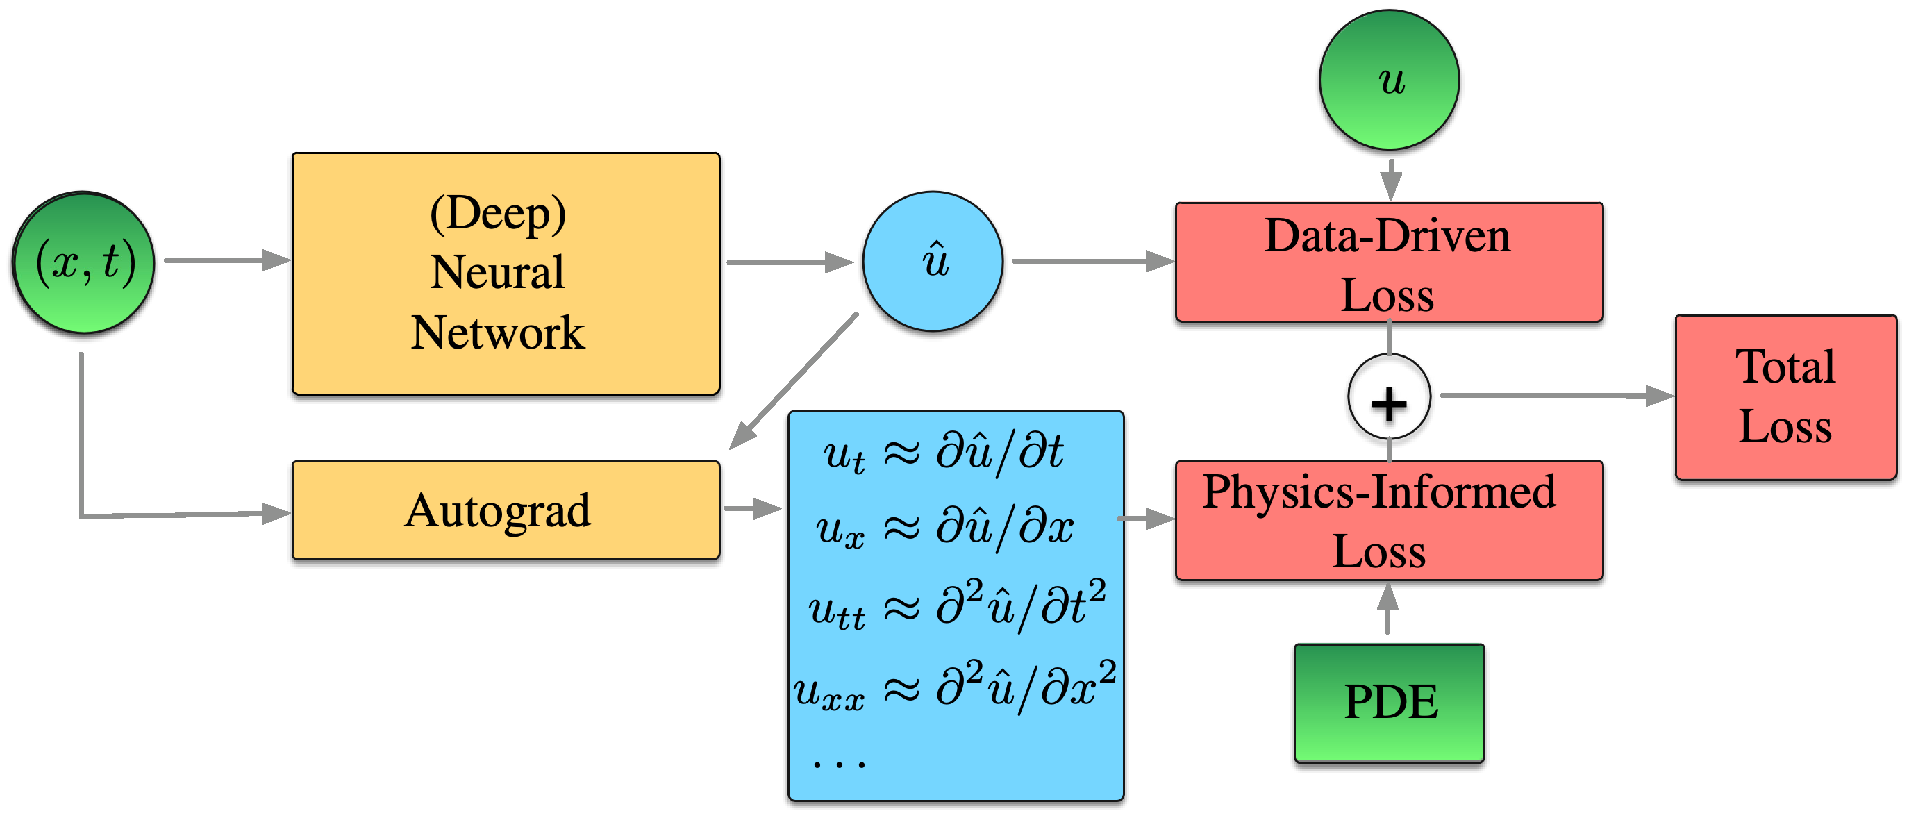
\includegraphics[width=1.05\textwidth]{graphics/PINN}
\par\end{center}

\rotatefoilhead{PINN - Diagram}
\begin{center}
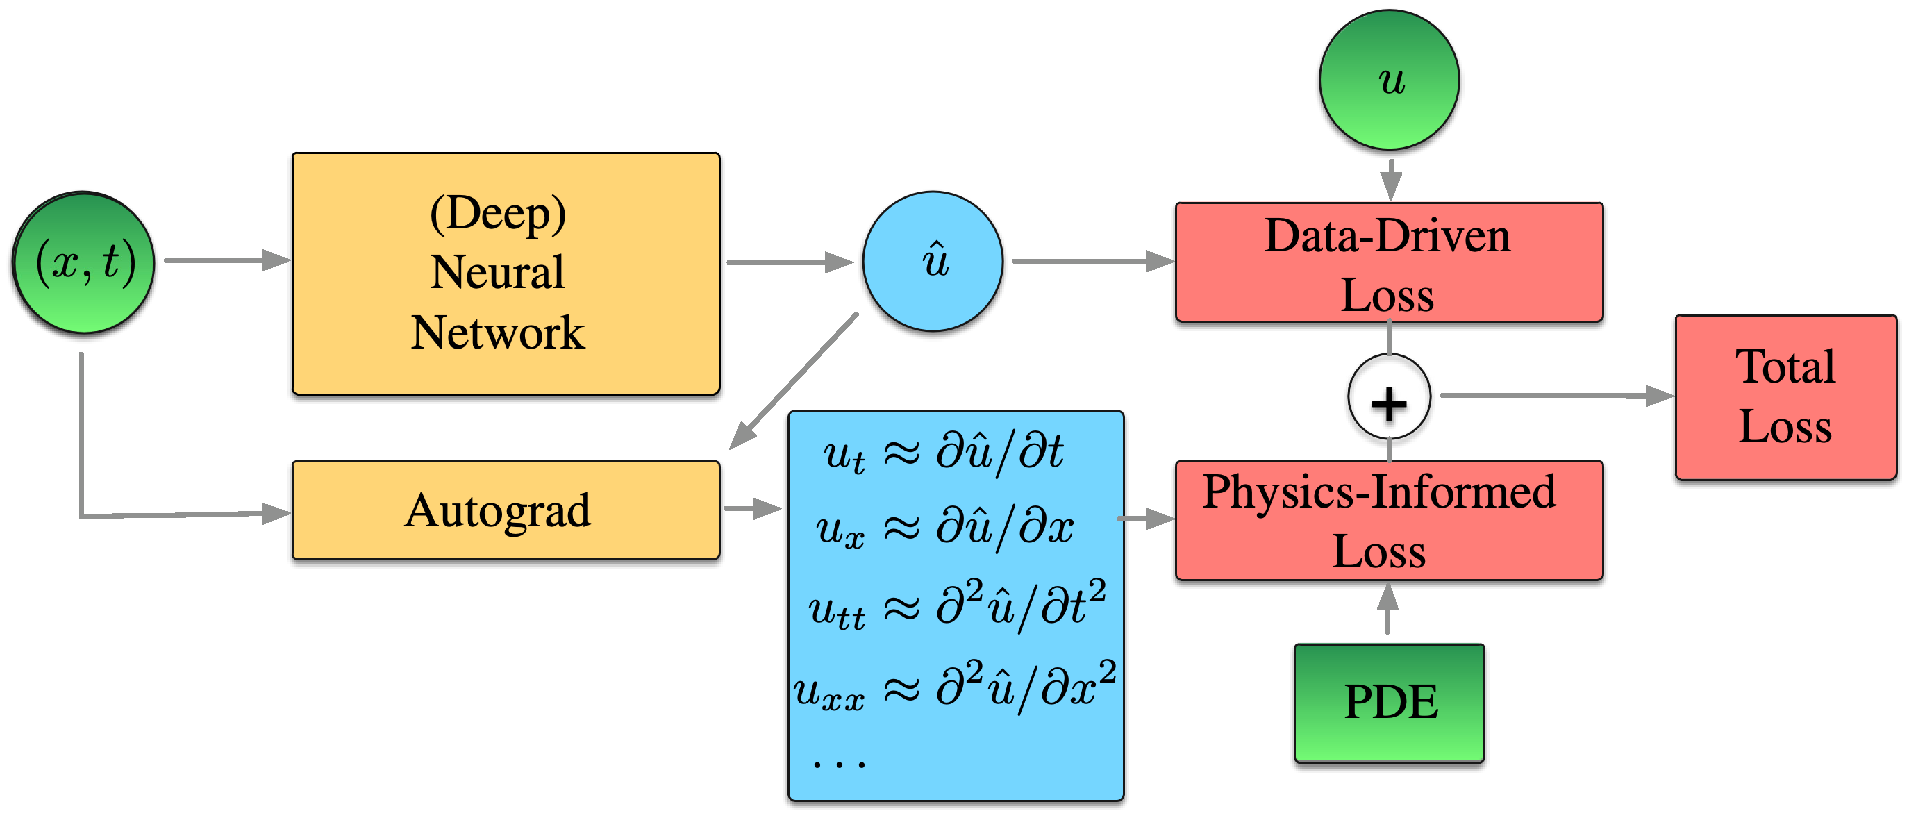
\includegraphics[width=1.05\textwidth]{graphics/PINN}
\par\end{center}

\foilhead{PINN Formulation - Neural Network}
\begin{itemize}
\item \textbf{Neural Network}: 
\begin{itemize}
\item a basic/adequate definition is to simply consider a NN as a mathematical
function with some \textcolor{magenta}{learnable parameters}
\item more mathematically, let the \textcolor{magenta}{network} be defined
as 
\[
\mathrm{NN}(\mathbf{x},\mathbf{\theta})\colon\mathbb{R}^{d_{x}}\times\mathbb{R}^{d_{\theta}}\times\mathbb{R}^{d_{u}}
\]
where
\begin{itemize}
\item $\mathbf{x}$ are the inputs to the network
\item $\mathbf{\theta}$ are a set of learnable paramaters (usually, weights)
\item $d_{x},$ $d_{\theta}$ and $d_{u}$ are the dimensions of the network's
inputs, parameters and outputs, respectively.
\end{itemize}
\item The exact form of the network function is determined by the neural
network\textquoteright s \textcolor{magenta}{architecture}. Here we
use feedforward fully-connected networks (FCNNs), defined as
\[
\mathrm{NN}(\mathbf{x},\mathbf{\theta})=f_{n}\circ\cdots\circ f_{i}\circ\cdots\circ f_{1}(\mathbf{x},\mathbf{\theta}),
\]
 where
\begin{itemize}
\item $\mathbf{x}\in\mathbb{R}^{d_{0}}$ is the input to the FCNN
\item $\mathrm{NN}\in\mathbb{R}^{d_{n}}$ is the output of the FCNN
\item $n$ is the number of layers (depth) of the FCNN
\item $f_{i}(\mathbf{x},\mathbf{\mathbf{\theta}})=\sigma_{i}(W_{i}\mathbf{x}+\mathbf{b})$
are element-wise, nonlinear activation functions (usually ReLU or
hyperbolic tangent)
\item with $\theta_{i}=(W_{i},\mathbf{b}_{i}),$
\item $W_{i}\in\mathbb{R}^{d_{i}\times d_{i-1}}$ weight matrices, $\mathbf{b}\in\mathbb{R}^{d_{i}}$
bias vectors, and
\item $\mathbf{\mathbf{\theta}}=(\mathbf{\mathbf{\theta}}_{1},\ldots,\mathbf{\mathbf{\theta}}_{i},\ldots,\mathbf{\mathbf{\theta}}_{n})$
are the s et of learnable parameters/weights of the network.
\end{itemize}
\end{itemize}
\end{itemize}

\foilhead{Recall: FCNN Architecture and Activation}
\begin{center}
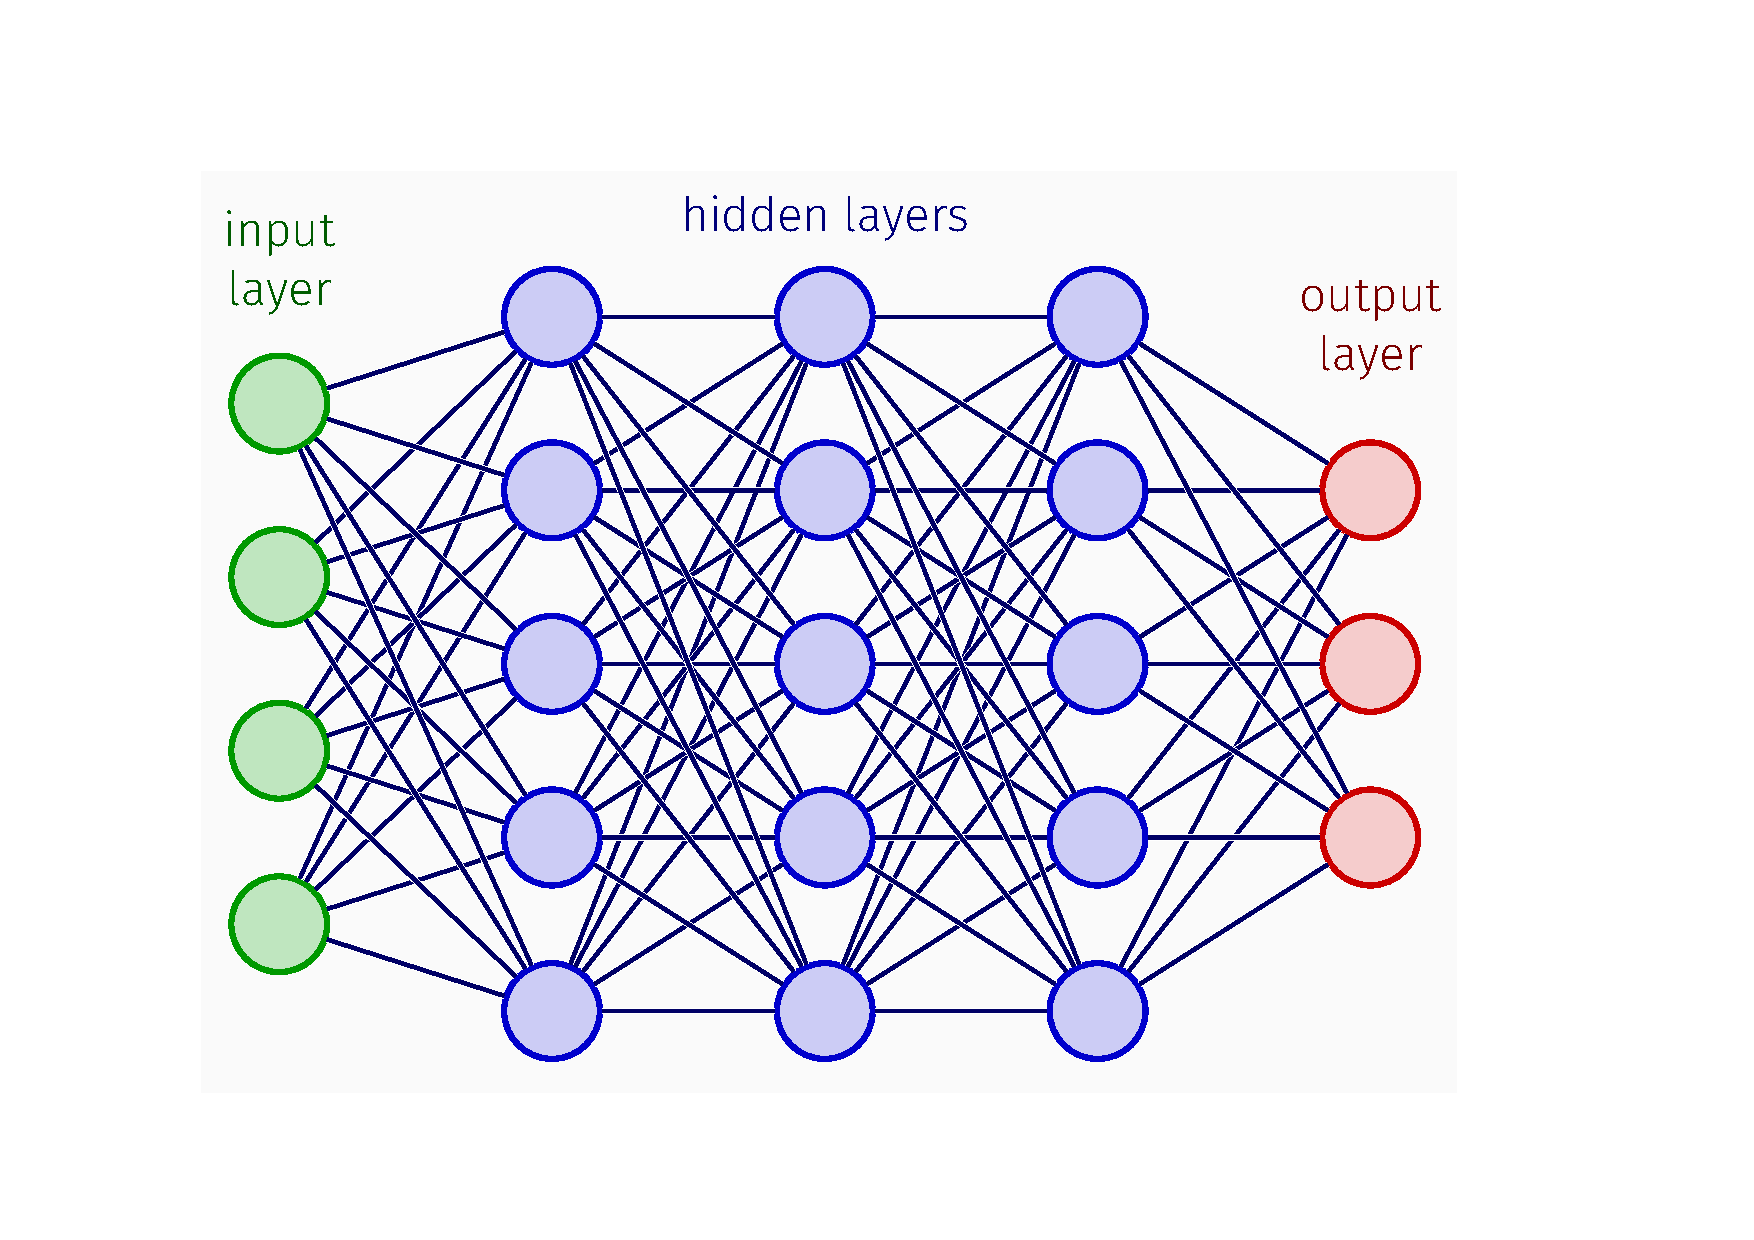
\includegraphics[width=1.05\textwidth]{graphics/FCNN_tikz}
\par\end{center}

\begin{center}
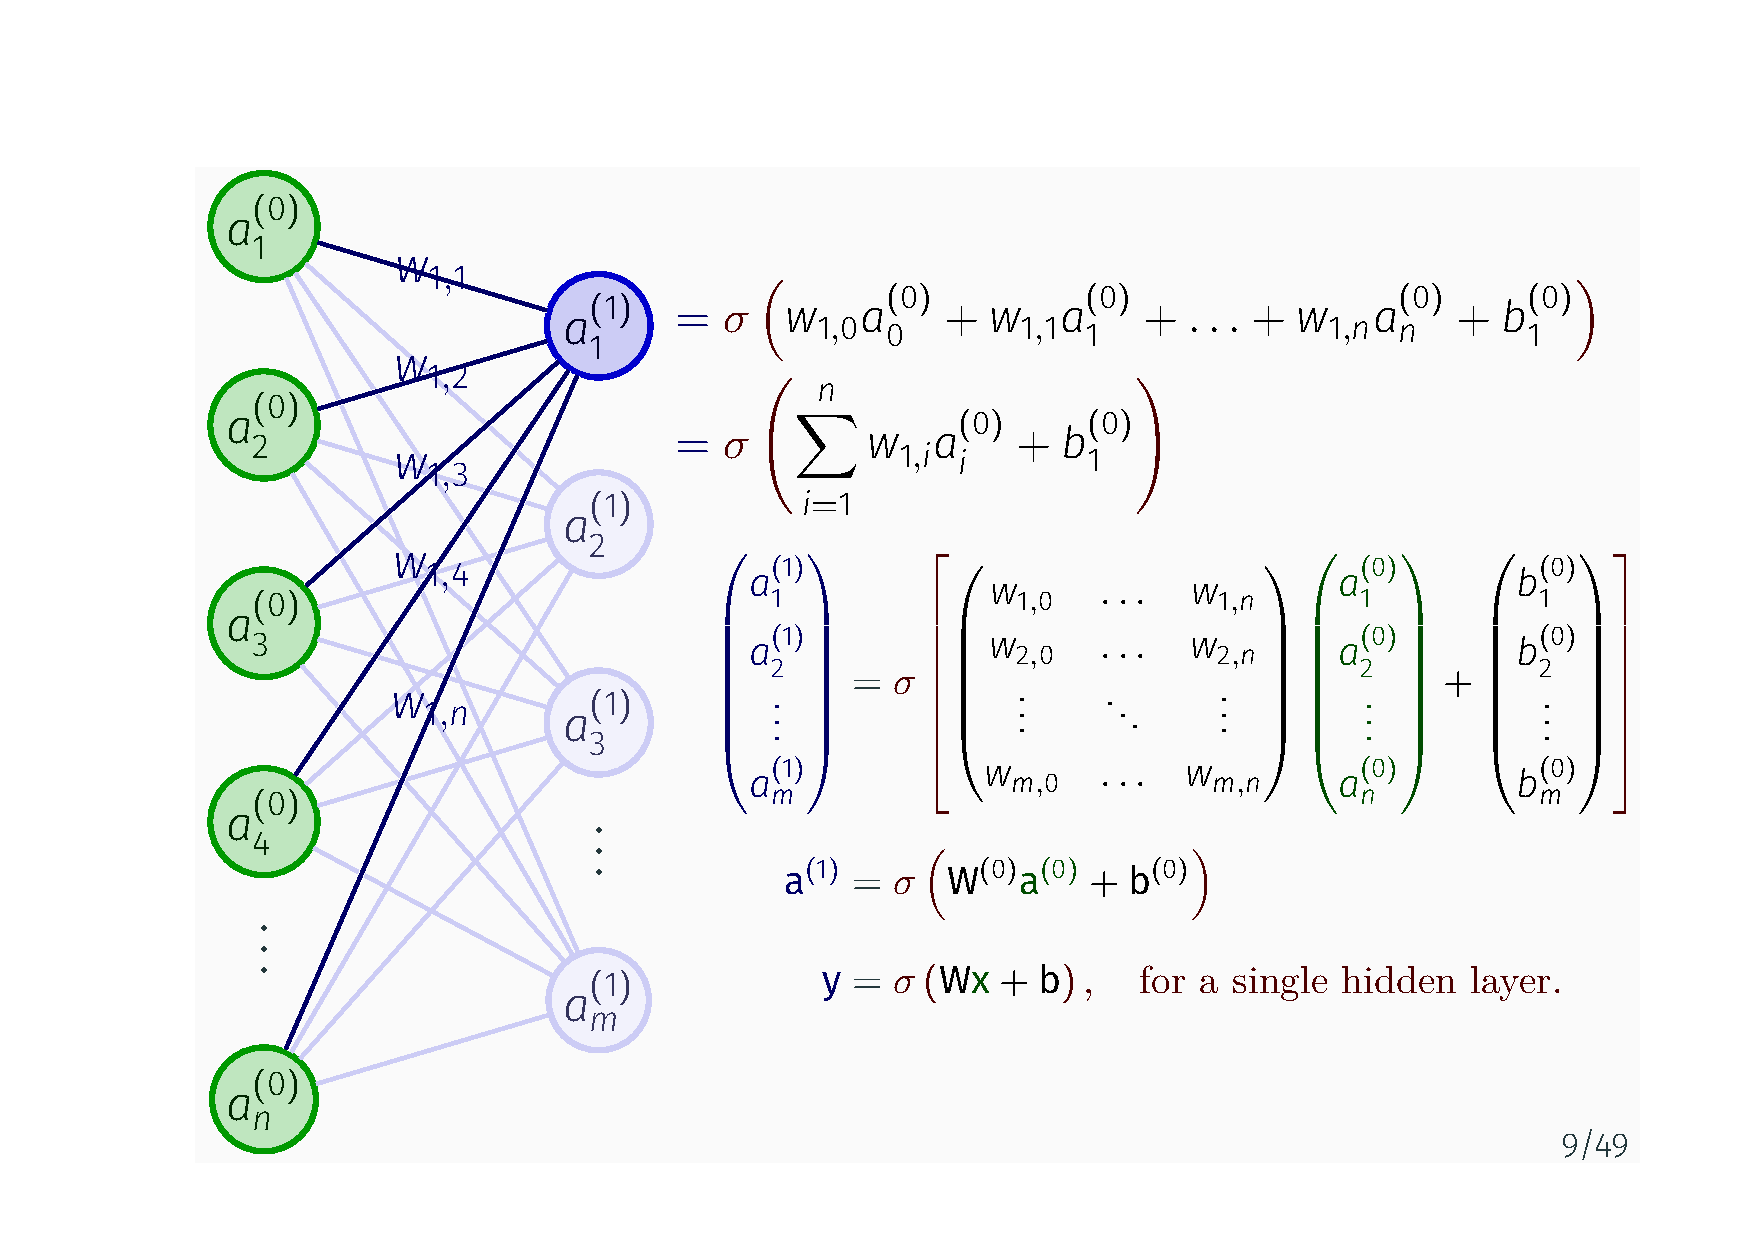
\includegraphics[width=1.05\textwidth]{graphics/FCNN_activ}
\par\end{center}

\foilhead{PINN Formulation - (P)DE}
\begin{itemize}
\item Recall: PINNs use neural networks to solve problems related to differential
equations
\item Consider a general \textcolor{magenta}{boundary-value problem} (I)BVP
of the form
\begin{align}
\mathcal{D}[u](\mathbf{\mathrm{x}}) & =f(\mathbf{\mathrm{x}}),\quad\mathbf{\mathrm{x}}\in\Omega\subset\mathbb{R}^{d},\label{eq:(P)DE}\\
\mathcal{B}_{k}[u](\mathbf{\mathrm{x}}) & =g_{k}(\mathbf{\mathrm{x}}),\quad\mathbf{\mathrm{x}}\in\Gamma_{k}\subset\partial\Omega,\nonumber 
\end{align}
where
\begin{itemize}
\item $\mathcal{D}[u](\mathbf{\mathrm{x}})$ is a differential operator
\item $u(\mathbf{\mathrm{x}})$ is the solution
\item $\mathcal{B}_{k}(\cdot)$ are a set of boundary and/or initial conditions
that ensure uniqueness of the solution
\item the variable $\mathbf{\mathrm{x}}$ represents/includes both spatial
and time variables
\item the full equation describes many possible contexts: linear and nonlinear,
time-dependent and independent, irregular higher-order, cyclic BCs,
etc.
\item To solve (\ref{eq:(P)DE}), PINNs use a neural network to directly
approximate the solution,
\[
\mathrm{NN}(\mathbf{x},\mathbf{\theta})\approx u(\mathbf{x})
\]
\end{itemize}
\item PINN provides a \textcolor{magenta}{functional approximation} to the
solution, and not a discretized solution similar to that provided
by traditional methods such as finite difference methods 
\begin{itemize}
\item as such PINNs are a \textcolor{magenta}{mesh-free} approach for solving
differential equations
\end{itemize}
\end{itemize}

\foilhead{PINN Formulation - Loss Function}
\begin{itemize}
\item \textbf{Loss Function}: Let $F=0$ be the PDE, $B=0$ the boundary/initial
conditions, $I=0$ the \textcolor{magenta}{inversion} conditions,
then the PINN loss is
\[
\mathcal{L}(\theta,\lambda;\mathcal{T})=w_{f}\mathcal{L}_{f}(\theta,\lambda;\mathcal{T}_{f})+w_{b}\mathcal{L}_{b}(\theta\lambda;\mathcal{T}_{b})+\textcolor{magenta}{w_{i}\mathcal{L}_{i}(\theta,\lambda;\mathcal{T}_{i})}
\]
 where
\begin{align*}
\mathcal{L}_{f}(\theta;\mathcal{T}_{f}) & =\left\Vert F(\hat{u},x,\lambda)\right\Vert _{2}^{2}\\
\mathcal{L}_{b}(\theta;\mathcal{T}_{b}) & =\left\Vert B(\hat{u},x)\right\Vert _{2}^{2}\\
\textcolor{magenta}{\mathcal{L}_{i}(\theta,\lambda,\mathcal{T}_{i})} & =\frac{1}{\left|\mathcal{T}_{i}\right|}\sum_{x\in\mathcal{T}_{i}}\left\Vert I(\hat{u},x)\right\Vert _{2}^{2}
\end{align*}
 and
\begin{itemize}
\item $x$ are the training points, 
\item $\hat{u}$ the approximate solution, 
\item $\textcolor{magenta}{\lambda}$ the inversion coefficients,
\item $w$ the weights that ensure balance among the different loss function
terms
\item $\mathcal{T}$ are the sets of training points for each loss term 
\end{itemize}
\item The solution is then given by, 
\[
\left\{ \theta^{*},\textcolor{magenta}{\lambda}^{*}\right\} =\argmin_{\theta,\textcolor{magenta}{\lambda}}\mathcal{L}(\theta,\textcolor{magenta}{\lambda};\mathcal{T})
\]
\item \textbf{Note}: solving the inverse problems requires only the addition
of one term in the loss function, and nothing more!
\end{itemize}

\foilhead{PINN Formulation - Error Analysis}
\begin{itemize}
\item Error analysis can been derived\footnote{Lu, Karniadakis, SIAM Review, 2021.}\footnote{Mishra, Molinaro; arXiv:2006.16144v2 and IMA J. of Numerical Analysis,
Volume 43, Issue 1, January 2023, Pages 1--43.}, in terms of 
\begin{itemize}
\item optimization error $e_{o}=\left\Vert \hat{u}_{\mathcal{T}}-u_{\mathcal{T}}\right\Vert $
\item generalization error $e_{g}=\left\Vert u_{\mathcal{T}}-u_{\mathcal{F}}\right\Vert $
\item approximation error $e_{a}=\left\Vert u_{\mathcal{F}}-u\right\Vert $
\end{itemize}
\item then
\[
e\doteq\left\Vert \hat{u}_{\mathcal{T}}-u\right\Vert \le e_{o}+e_{g}+e_{a}
\]
\end{itemize}

\foilhead{PINN Formulation - Loss Function (II)}
\begin{itemize}
\item The values for the loss function are available, in general, at \textcolor{magenta}{discrete}
points, often called \textcolor{magenta}{collocation} points.
\item We will write down the terms explicitly in this case, for the direct
problem, with composite loss function,
\begin{equation}
\mathcal{L}(\mathbf{\theta})=\mathcal{L}_{D}(\mathbf{x},\mathbf{\theta})+\mathcal{L}_{B}(\mathbf{x},\mathbf{\theta}),\label{eq:loss}
\end{equation}
where
\begin{itemize}
\item \textcolor{magenta}{(P)DE residual} is defined as
\[
\mathcal{L}_{D}(\mathbf{x},\mathbf{\theta})=\frac{\alpha_{I}}{N_{I}}\sum_{i=1}^{N_{I}}\left(\mathcal{D}[u](\mathbf{\mathrm{x}}_{i},\mathbf{\theta})-f(\mathbf{\mathrm{x}}_{i})\right)^{2}
\]
\item \textcolor{magenta}{(I)BC residual} is defined as
\[
\mathcal{L}_{B}(\mathbf{x},\mathbf{\theta})=\sum_{k=1}^{N_{k}}\frac{\alpha_{B}^{k}}{N_{B}^{k}}\sum_{i=1}^{N_{B}^{k}}\left(\mathcal{B}_{k}[u](\mathbf{\mathrm{x}}_{i}^{k},\mathbf{\theta})-g_{k}(\mathbf{\mathrm{x}}_{i}^{k})\right)^{2},
\]
 where
\begin{itemize}
\item $\left\{ \mathbf{\mathrm{x}}_{i}\right\} _{i=1}^{N_{I}}$ is a set
of \textcolor{magenta}{collocation} points sampled in the \textcolor{magenta}{interior}
of the domain
\item $\left\{ \mathbf{\mathrm{x}}_{j}^{k}\right\} _{j=1}^{N_{B}^{k}}$
is a set of points sampled along each \textcolor{magenta}{boundary
condition }(where $k$ permits to separate Dirichlet, Neumann, mixed,
and initial conditions)
\item $\alpha_{I}$ and $\alpha_{B}^{k}$ are well-chosen scalar \textcolor{magenta}{weights},
chosen by suitable \textcolor{magenta}{tuning} methods, that ensure
the terms in the loss function are \textcolor{magenta}{well-balanced}.
\end{itemize}
\end{itemize}
\end{itemize}

\foilhead{PINN Formulation - Loss Function (III)}

We can see, intuitively, that 
\begin{itemize}
\item by minimizing the \textcolor{magenta}{(P)DE residual}, the method
tries to ensure that the solution learned by the network obeys the
underlying PDE, and 
\item by minimizing the\textcolor{magenta}{{} (I)BC residual}, the method
tries to ensure that the learned solution is unique by matching it
to the BCs. 
\item \textbf{Note}: a sufficient number of collocation and boundary points
must be chosen such that the PINN is able to learn a consistent solution
across the domain.
\end{itemize}
As usual (see \textcolor{blue}{Optimization Lecture)}, iterative schemes
are typically used to optimize this loss function
\begin{itemize}
\item variants of the stochastic gradient descent (SGD) method, such as
the Adam optimizer, or 
\item quasi-Newton methods, such as the limited-memory Broyden--Fletcher--Goldfarb--Shanno
(L-BFGS) algorithm are employed. 
\end{itemize}
\textbf{Note}: 
\begin{itemize}
\item These methods require the computation of the gradient of the loss
function with respect to the network parameters, which can computed
easily and efficiently using \textcolor{magenta}{automatic differentiation}
provided systematically in all modern deep learning libraries 
\item Note also that gradients of the network output with respect to its
inputs are also typically required to evaluate the \textcolor{magenta}{PDE
residual }in the loss function, and can similarly be obtained and
further differentiated through to update the network\textquoteright s
parameters using \textcolor{magenta}{automatic differentiation} once
again.
\end{itemize}
Recall the global flowchart for PINN:
\begin{center}
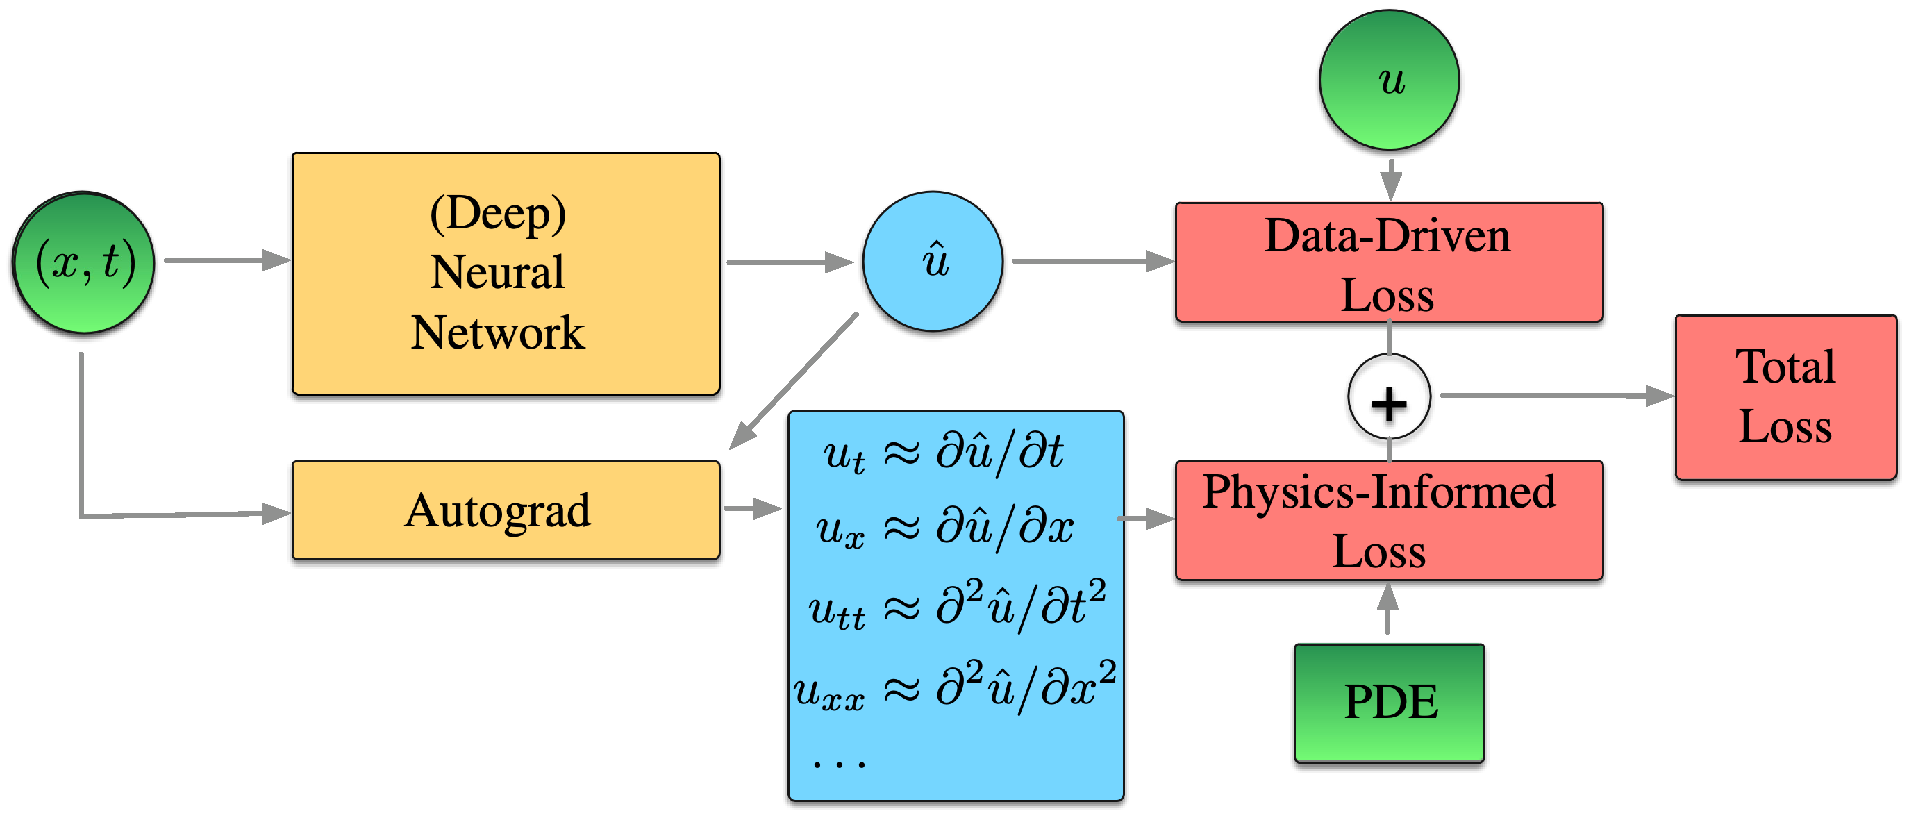
\includegraphics[width=1.05\textwidth]{graphics/PINN}
\par\end{center}

Here is a case with 2 hidden layer NN:
\begin{center}
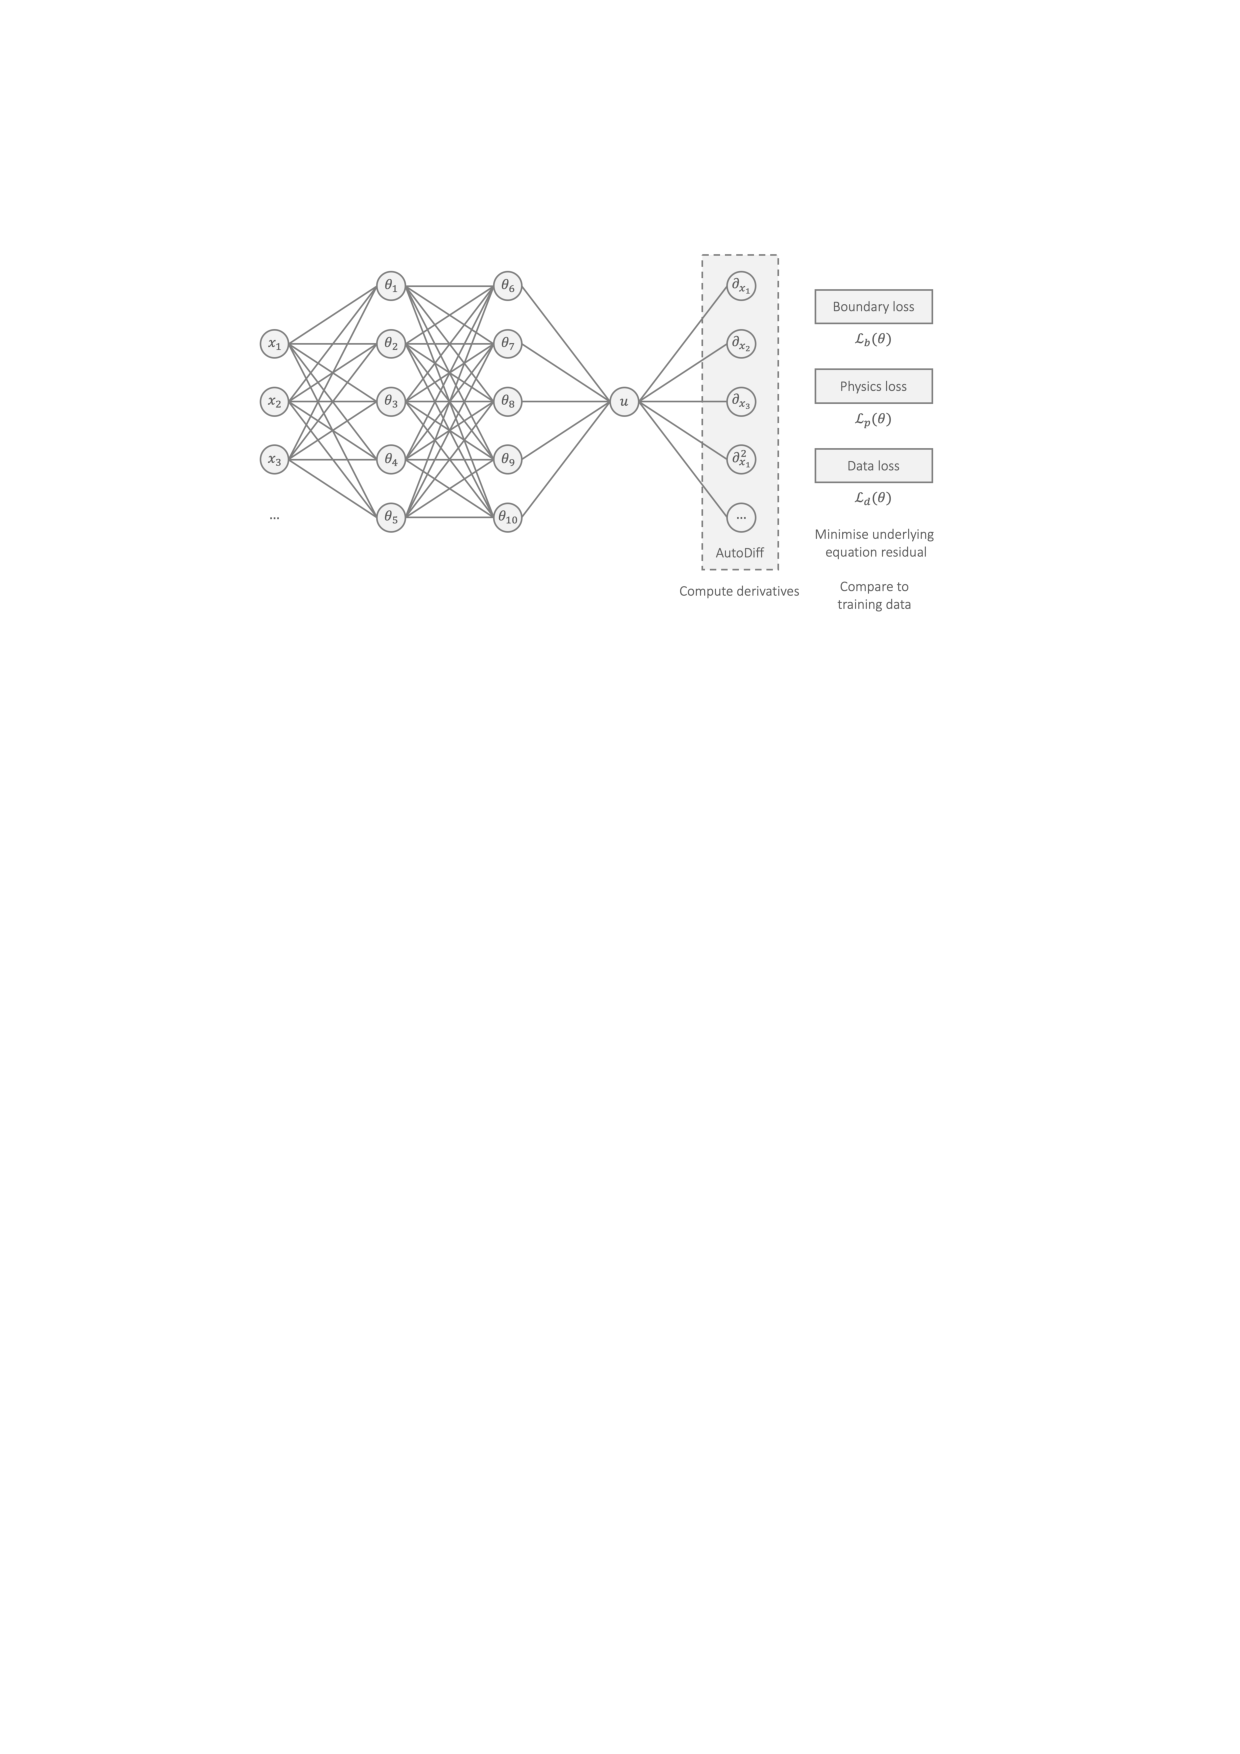
\includegraphics[width=0.8\textwidth]{graphics/simplePINN}
\par\end{center}

\foilhead{PINN - pros and cons}
\begin{itemize}
\item Here are some of the \textcolor{magenta}{advantages} of using PINNs
to solve differential equations:
\begin{dinglist}{52}
\item They can be used to solve a wide variety of differential equations,
including ODEs and PDEs.
\item They can be used to solve problems with complex geometries and non-linear
behavior. 
\item They are essentially mesh-free.
\item They can be trained to be very accurate, even with limited data and
noisy data.
\item They are relatively easy to implement, leveraging AD capabilities. 
\item When they work, they can provide impressive speed-ups of 3 to 4 orders
of magnitude.
\end{dinglist}
\item Here are some of the \textcolor{magenta}{disadvantages} of using PINNs
to solve differential equations:
\begin{dinglist}{56}
\item They can produce a horrendous optimization problem.
\item They can be computationally expensive to train.
\item They have difficulty with high frequencies and multiple scales. 
\item They can be sensitive to the choice of hyperparameters, in particular
to the network architecture and size.
\item They can be difficult to interpret, as the neural network may learn
a complex relationship between the inputs and outputs that is not
easily understood.
\end{dinglist}
\item Overall, PINNs are a \textcolor{magenta}{promising} new approach to
solving differential equations. 
\begin{itemize}
\item They provide powerful tools that can be used to solve a wide variety
of problems, but they also have some severe limitations.
\end{itemize}
\end{itemize}

\foilhead{PINN - remedies}
\begin{itemize}
\item A downside of training PINNs with the loss function given by (\ref{eq:loss})
is that the BCs are \textcolor{magenta}{softly} enforced. 
\begin{itemize}
\item This means the \textcolor{magenta}{learned solution may deviate} from
the BCs because the BC term may not be fully minimized. 
\item Furthermore, it can be challenging to \textcolor{magenta}{balance
the different objectives} of the PDE and BC terms in the loss function,
which can lead to \textcolor{magenta}{poor convergence }and solution
accuracy.
\end{itemize}
\item One possibility is to enforce BCs in a \textcolor{magenta}{hard }fashion
by using the neural network as part of a solution \emph{ansatz}. This
will be shown in some of the examples below.
\item Many other ``fixes'' have been formulated (see references, in particular
arXiv, where new solutions appear almost daily...)
\end{itemize}

\foilhead{PINN Remedies - enforcing hard BCs}
\begin{itemize}
\item \textbf{Idea}: use the NN as part of a solution ansatz, that by definition
satisfies the BC, thus avoiding the soft constraint on $\mathcal{L}_{B}$
in (\ref{eq:loss})
\item More precisely, we approximate the solution of the (P)DE by
\[
\mathcal{C}[u](\mathbf{\mathrm{x}},\mathbf{\theta})\approx u(\mathbf{\mathrm{x}},\mathbf{\theta})
\]
 where $\mathcal{C}$ is an appropriately selected constraining operator
that analytically/exactly enforces the BCs
\item \textbf{Example}: 
\begin{itemize}
\item suppose we want to enforce
\[
u(x=0)=0
\]
 in a scalar ODE
\item The constraining operator and solution ansatz could be chosen as 
\[
\mathcal{C}[u](\mathbf{\mathrm{x}},\mathbf{\theta})=\left(\tanh x\right)u(\mathbf{\mathrm{x}},\mathbf{\theta})
\]
 or any other function whose value at $x=0$ is zero
\begin{itemize}
\item the function $\tanh(x)$ is zero at 0, \textcolor{magenta}{forcing}
the BC to always be obeyed, but non-zero away from 0, allowing the
network to learn the solution away from the BC.
\end{itemize}
\end{itemize}
\item With this approach, the BCs are always satisfied and therefore the
BC term in the loss function (\ref{eq:loss}) can be removed, 
\begin{itemize}
\item the PINN can be trained using the simpler unconstrained loss function,
\[
\mathcal{L}(\mathbf{\theta})=\frac{1}{N}\sum_{i=1}^{N}\left(\mathcal{D}[\mathcal{C}u](\mathbf{\mathrm{x}}_{i},\mathbf{\theta})-f(\mathbf{\mathrm{x}}_{i})\right)^{2}
\]
where $\left\{ \mathbf{\mathrm{x}}_{i}\right\} _{i=1}^{N}$ is a set
of \textcolor{magenta}{collocation} points sampled in the \textcolor{magenta}{interior}
of the domain
\end{itemize}
\item \textbf{Notes}: 
\begin{itemize}
\item There is no unique way of choosing the constraining operator, and
the definition of a suitable constraining operator for complex geometries
and/or complex BCs may be difficult or sometimes even impossible,
i.e., this strategy is problem dependent; in this case, one may resort
to the soft enforcement of boundary conditions (\ref{eq:loss}) instead.
\item A promising approach for alleviating the difficulties when higher
frequencies and multi-scale features are added to the solution, is
to use a finite basis PINN approach (FBPINN) {[}Dolean, Heinlein,
Mishra, Moseley 2023{]}, where instead of using a single neural network
to represent the solution, many smaller neural networks are confined
in overlapping subdomains and summed together to represent the solution.
\end{itemize}
\end{itemize}

\foilhead{Example: IBVP for Diffusion Equation}

\textbf{Compute} $u(\mathbf{x},t)\colon\Omega\times[0,T]\rightarrow\mathbb{R}$
such that 
\begin{align}
\frac{\partial u(\mathbf{x},t)}{\partial t}-\nabla\cdot\left(\lambda(x)\nabla u(\mathbf{x},t)\right) & =f(\mathbf{x},t)\mathrm{\quad in\,\,\Omega\times(0,T),}\label{eq:ibvp-pde}\\
u(\mathbf{x},t) & =g_{D}(\mathbf{x},t)\mathrm{\quad on\,\,\partial\Omega_{D}\times(0,T),}\nonumber \\
-\lambda(x)\nabla u(\mathbf{x},t)\cdot\mathbf{n} & =g_{R}(\mathbf{x},t)\mathrm{\quad on\,\,\partial\Omega_{R}\times(0,T),}\nonumber \\
u(\mathbf{x},0) & =u_{0}(\mathbf{x})\mathrm{\quad for\,\,x\in\Omega.}\nonumber 
\end{align}
Note that $\lambda(x)$ is, in general, a tensor (matrix) with elements
$\lambda_{ij}.$
\begin{itemize}
\item \textbf{\textcolor{magenta}{Direct}}\textbf{ problem}: given $\lambda,$
compute $u.$
\item \textbf{\textcolor{magenta}{Inverse}}\textbf{ problem}: given $u,$
compute $\lambda.$
\end{itemize}

\foilhead{PINN for the Diffusion Equation}

\includegraphics[scale=1.35]{../../../../../../1Research/Glotin/talks/PNN-heat}

{\tiny{[}Credit: Lu, Karniadakis, SIAM Review, 2021{]}}{\tiny\par}
\begin{itemize}
\item Use \textcolor{magenta}{FCNN} to approximate $u$ at the selected
points $x,$ with training data at residual points $\mathcal{T}_{f}$
and $\mathcal{T}_{b}$
\item Use \textcolor{magenta}{AD} to compute derivatives for the PDE and
the boundary/initial conditions
\item \textcolor{magenta}{Minimize} the augmented, weighted loss function 
\end{itemize}

\foilhead{$\;$}

\vfill{}

\begin{center}
{\Large\textbf{\textcolor{blue}{PHYSICS OPERATOR LEARNING}}}{\Large\par}
\par\end{center}

\vfill{}


\foilhead{Recall: Universal Approximation for Operators}
\begin{thm}
[Chen, Chen 1995]Suppose $\sigma$ is continuous, non-polynomial,
$X$ is a Banach space, $K_{1}\subset X,$ $K_{2}\subset\mathbb{R}^{d}$
are compact sets, $V$ is compact in $C(K_{1}),$ $G$ is continuous
operator from $V$ into $C(K_{2}).$ Then, for any $\epsilon>0,$
there exist positive integers $m,$ $n,$ $p,$ constants $c_{k}^{i},$
$\xi_{ij}^{k},$ $\theta_{i}^{k},$ $\zeta_{k}\in\mathbb{R},$ $w_{k}\in\mathbb{R}^{d},$
$x_{j}\in K_{1},$ such that
\begin{gather*}
\left|G(u)(y)-\sum_{k=1}^{p}\sum_{i=1}^{n}c_{i}^{k}\sigma\left(\sum_{j=1}^{m}\xi_{ij}^{k}u(x_{j})+\theta_{i}^{k}\right)\sigma\left(w_{k}\cdot y+\zeta_{k}\right)\right|\\
<\epsilon
\end{gather*}
 for all $u\in V,$ $y\in K_{2}.$ 
\end{thm}

\foilhead{Operator Learning - DeepONet, FNO, PINO}
\begin{itemize}
\item \textbf{Idea}: train a NN to learn the (P)DE operator
\begin{itemize}
\item used by NVIDIA in FourCastNet
\end{itemize}
\item A related set of approaches which incorporate governing equations
into their loss function are physics-informed neural operators (PINO). 
\item These are neural networks which are similar to PINNs in that they
are designed to learn the solution to differential equations, but
instead of learning a single solution they learn an entire \textcolor{magenta}{family
of solutions }by adding certain inputs of the differential equation
as inputs to the network. 
\item Thus, they do not need to be retrained to carry out new simulations,
and during inference they offer a fast surrogate model. 
\item From a mathematical standpoint, the goal is to learn an \textcolor{magenta}{operator}
to map function spaces to function spaces, rather than just a single
function.
\item \textcolor{magenta}{DeepONet} consisted of two sub-networks, 
\begin{itemize}
\item a \textquotedblleft \textcolor{magenta}{branch}\textquotedblright{}
network that encodes the input function (by taking discretised samples
of the input function at fixed locations as input), and 
\item a \textquotedblleft \textcolor{magenta}{trunk}\textquotedblright{}
network that encodes a set of input coordinates. 
\item The solution of the differential equation is then approximated by
merging the outputs of both of these sub-networks. 
\item The network is trained using a loss function that extends the PINN
loss function (\ref{eq:loss}) by averaging over many random samples
of the input function.
\end{itemize}
\item \textcolor{magenta}{FNO} (Fourier Neural Operator) uses a physics-informed
loss function when training Fourier neural operators 
\begin{itemize}
\item Similar to DeepONets, FNOs learn an operator to map between function
spaces. 
\item This is achieved by using a series of stacked Fourier layers, where
the input to each layer is Fourier transformed and truncated to a
fixed number of Fourier modes. 
\item This truncation allows the model to learn mappings that are invariant
to the number of discrete points used in its inputs and outputs. 
\end{itemize}
\end{itemize}

\foilhead{Operator Nets}
\begin{itemize}
\item Use the Universal \textcolor{magenta}{Operator} Approximation Theorem...{\small
\begin{gather*}
\left|G(u)(y)-\sum_{k=1}^{p}\sum_{i=1}^{n}c_{i}^{k}\underbrace{\sigma\left(\sum_{j=1}^{m}\xi_{ij}^{k}u(x_{j})+\theta_{i}^{k}\right)}_{\mathrm{branch}}\underbrace{\sigma\left(w_{k}\cdot y+\zeta_{k}\right)}_{\mathrm{trunk}}\right|\\
<\epsilon,
\end{gather*}
}where 
\begin{itemize}
\item $G$ is the \textcolor{magenta}{solution} operator, 
\item $u$ is an \textcolor{magenta}{input} function,
\item $x_{i}$ are ``\textcolor{magenta}{sensor}'' points,
\item $y$ are \textcolor{magenta}{random points} where we evaluate the
output function $G(u).$
\end{itemize}
\item 2 main contenders:
\begin{itemize}
\item DeepONet
\item Fourier Neural Operators (FNO)---a special case of DeepONet
\end{itemize}
\end{itemize}

\foilhead{DeepONet Architecture}
\begin{center}
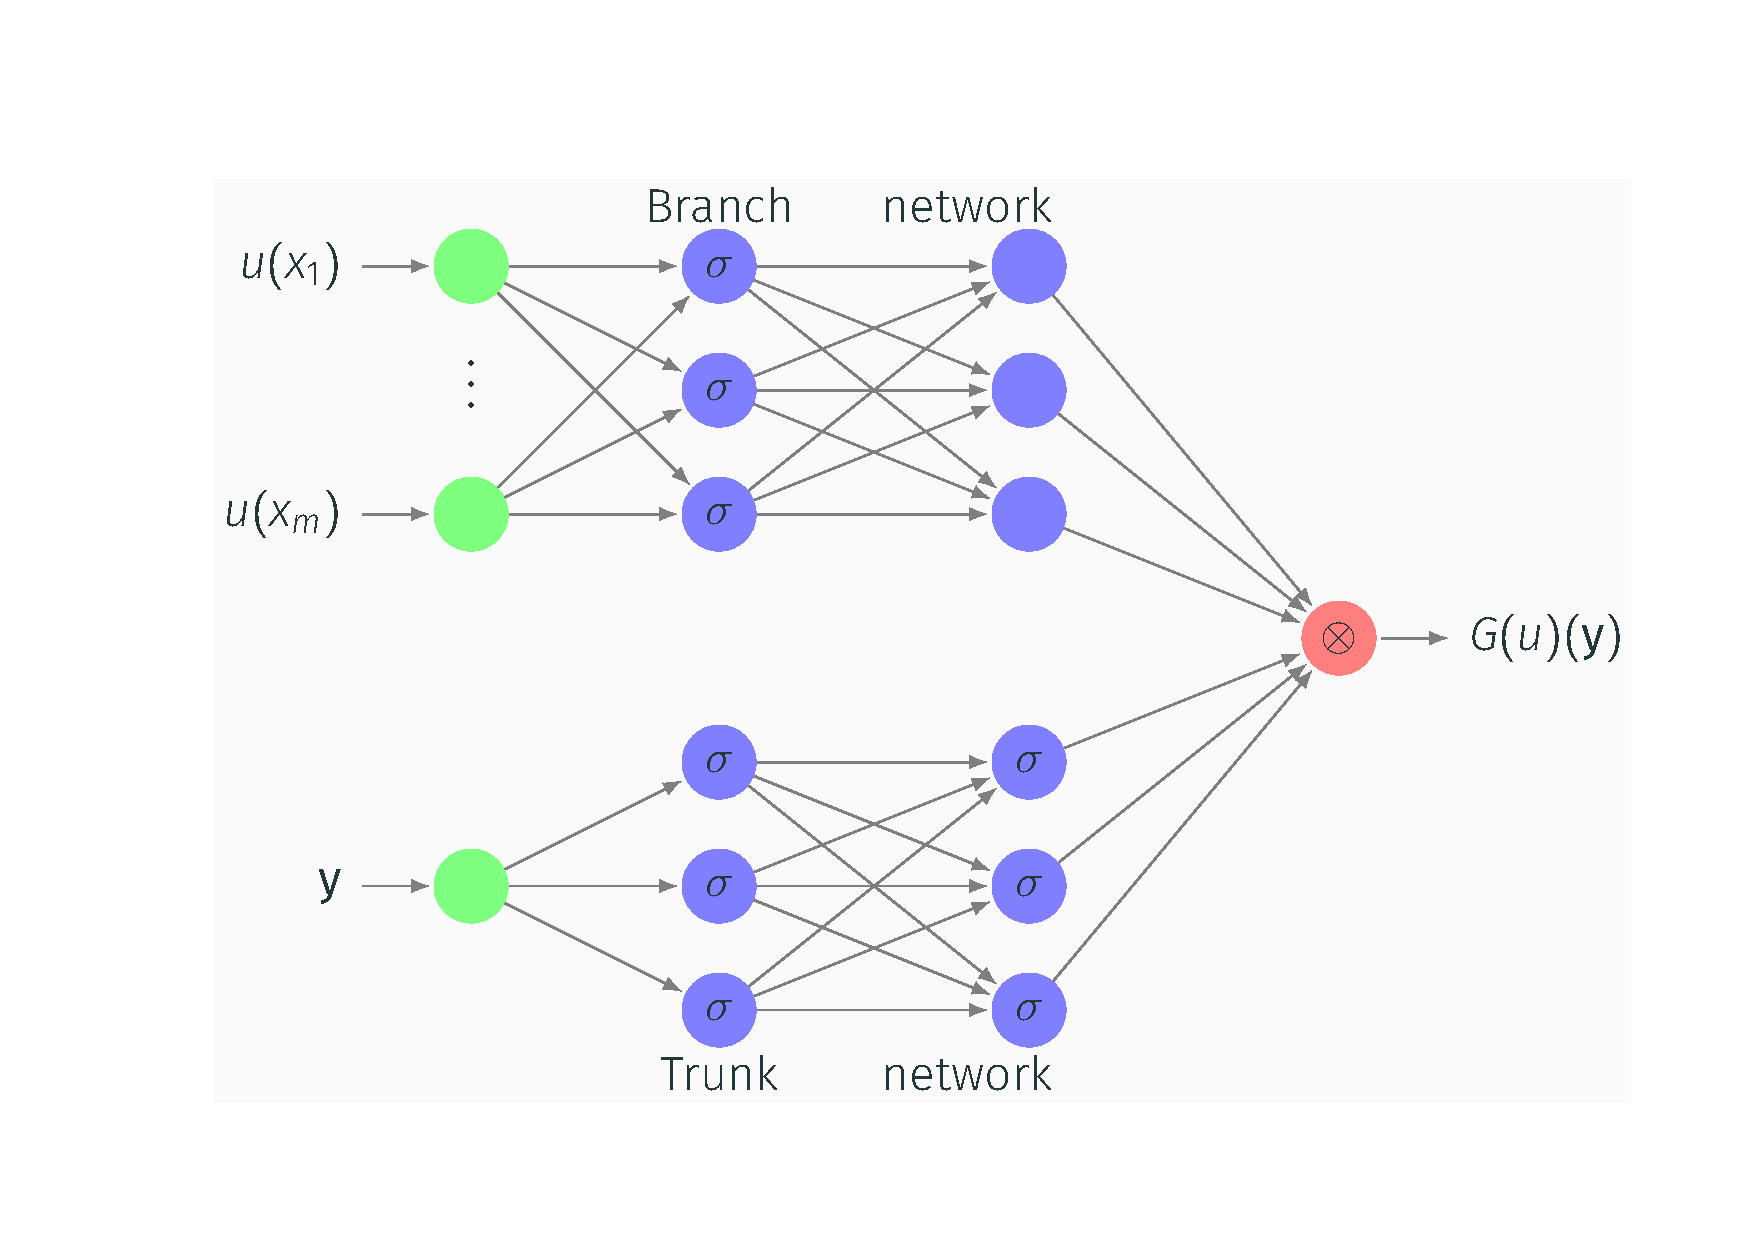
\includegraphics[width=1.05\textwidth]{graphics/deeponet_archi}
\par\end{center}

Directly copied from the Theorem!

\foilhead{DeepONet Loss Function}
\begin{itemize}
\item \textcolor{magenta}{Branch} (FCNN, ResNET, CNN, etc.) and \textcolor{magenta}{trunk}
networks (FCNN) are merged by an inner product.
\item \textcolor{magenta}{Prediction} of a function $u$ evaluated at points
$\mathbf{y}$ is then given by
\[
G_{\theta}(u)(y)=\sum_{k=1}^{q}\underbrace{b_{k}(u(x))}_{\mathrm{branch}}\underbrace{t_{k}(y)}_{\mathrm{trunk}}+b_{0}
\]
\item \textcolor{magenta}{Training} weights and biases, $\theta,$ computed
by \textcolor{magenta}{minimizing} the loss (mini-batch by Adam, single-batch
by L-BFGS) 
\[
\mathcal{L}_{o}(\theta)=\frac{1}{NP}\sum_{i=1}^{N}\sum_{j=1}^{P}\left|G_{\theta}(u^{(i)})(y_{j}^{(i)})-G(u^{(i)})(y_{j}^{(i)})\right|^{2}
\]
\end{itemize}

\foilhead{DeepONet: Pros and Cons}
\begin{itemize}
\item Pros:
\begin{dinglist}{52}
\item relatively \textcolor{magenta}{fast} training (compared to PINN)
\item can overcome the curse of \textcolor{magenta}{dimensionality} (in
some cases...)
\item suitable for \textcolor{magenta}{multiscale} and \textcolor{magenta}{multiphysics}
problems
\end{dinglist}
\item Cons:
\begin{dinglist}{56}
\item no guarantee that \textcolor{magenta}{physics} is respected
\item require \textcolor{magenta}{large} training sets of paired input-output
observations (expensive!)
\end{dinglist}
\end{itemize}

\foilhead{DeepONet Formulation (I)}
\begin{itemize}
\item Parametric, linear/nonlinear \textcolor{magenta}{operator plus IBC}
(IBVP)
\begin{align*}
\mathcal{O}(u,s) & =0,\\
\mathcal{B}(u,s) & =0,
\end{align*}
\item where
\begin{itemize}
\item $u\in\mathcal{U}$ is the input function (parameters),
\item $s\in\mathcal{S}$ is the hidden, solution function
\end{itemize}
\item If $\exists!$ solution $s=s(u)\in\mathcal{S}$ to the IBVP, then
we can define the \textcolor{magenta}{solution operator} $G\colon\mathcal{U}\mapsto\mathcal{S}$
by
\[
G(u)=s(u).
\]
\end{itemize}

\foilhead{DeepONet Formulation (II)}
\begin{itemize}
\item Approximate the solution map $G$ by a \textcolor{magenta}{DeepONet}
$G_{\theta}$ 
\[
G_{\theta}(u)(y)=\sum_{k=1}^{q}\underbrace{b_{k}(u(x))}_{\mathrm{branch}}\underbrace{t_{k}(y)}_{\mathrm{trunk}}+b_{0}
\]
where $\theta$ represents all the trainable weights and biases, computed
by minimizing the loss at a set of $P$ random output points $\left\{ y_{j}\right\} _{j=1}^{p}$
\[
\mathcal{L}(u,\theta)=\frac{1}{P}\sum_{j=1}^{P}\left|G_{\theta}(u)(y_{j})-s(y_{j})\right|^{2},
\]
 and $s(y_{j})$ is the PDE solution evaluated at $P$ locations in
the domain of $G(u)$
\end{itemize}

\foilhead{DeepONet Formulation (III)}
\begin{itemize}
\item To obtain a vector output, a \textcolor{magenta}{stacked version}
is defined by repeated sampling over $i=1,\ldots,N,$ giving the overall
operator loss
\[
\mathcal{L}_{o}(\theta)=\frac{1}{NP}\sum_{i=1}^{N}\sum_{j=1}^{P}\left|G_{\theta}(u^{(i)})(y_{j}^{(i)})-s^{(i)}(y_{j}^{(i)})\right|^{2}
\]
\end{itemize}

\foilhead{DeepONet + PINN = PI-DeepONet}
\begin{itemize}
\item We can combine the two, to get the best of both worlds
\[
\mathcal{L}(\theta)=w_{f}\mathcal{L}_{f}(G_{\theta}(u)(y))+w_{b}\mathcal{L}_{b}(G_{\theta}(u)(y))+\textcolor{magenta}{w_{o}\mathcal{L}_{o}(G_{\theta}(u)(y))}
\]
\item Results:\footnote{Wang, Wang, Bhouri, Perdikaris. arXiv:2103.10974v1, arXiv:2106.05384,
arXiv:2110.01654, arXiv:2110.13297}
\begin{itemize}
\item \textcolor{magenta}{no} need for paired input-ouput observations,
just samples of the input function and BC/IC (\textcolor{magenta}{self-supervised
learning})
\item respects the \textcolor{magenta}{physics}
\item improved predictive accuracy 
\item ideal for \textcolor{magenta}{parametric} PDE studies---optimization,
parameter estimation, screening, etc.
\end{itemize}
\end{itemize}
\begin{center}
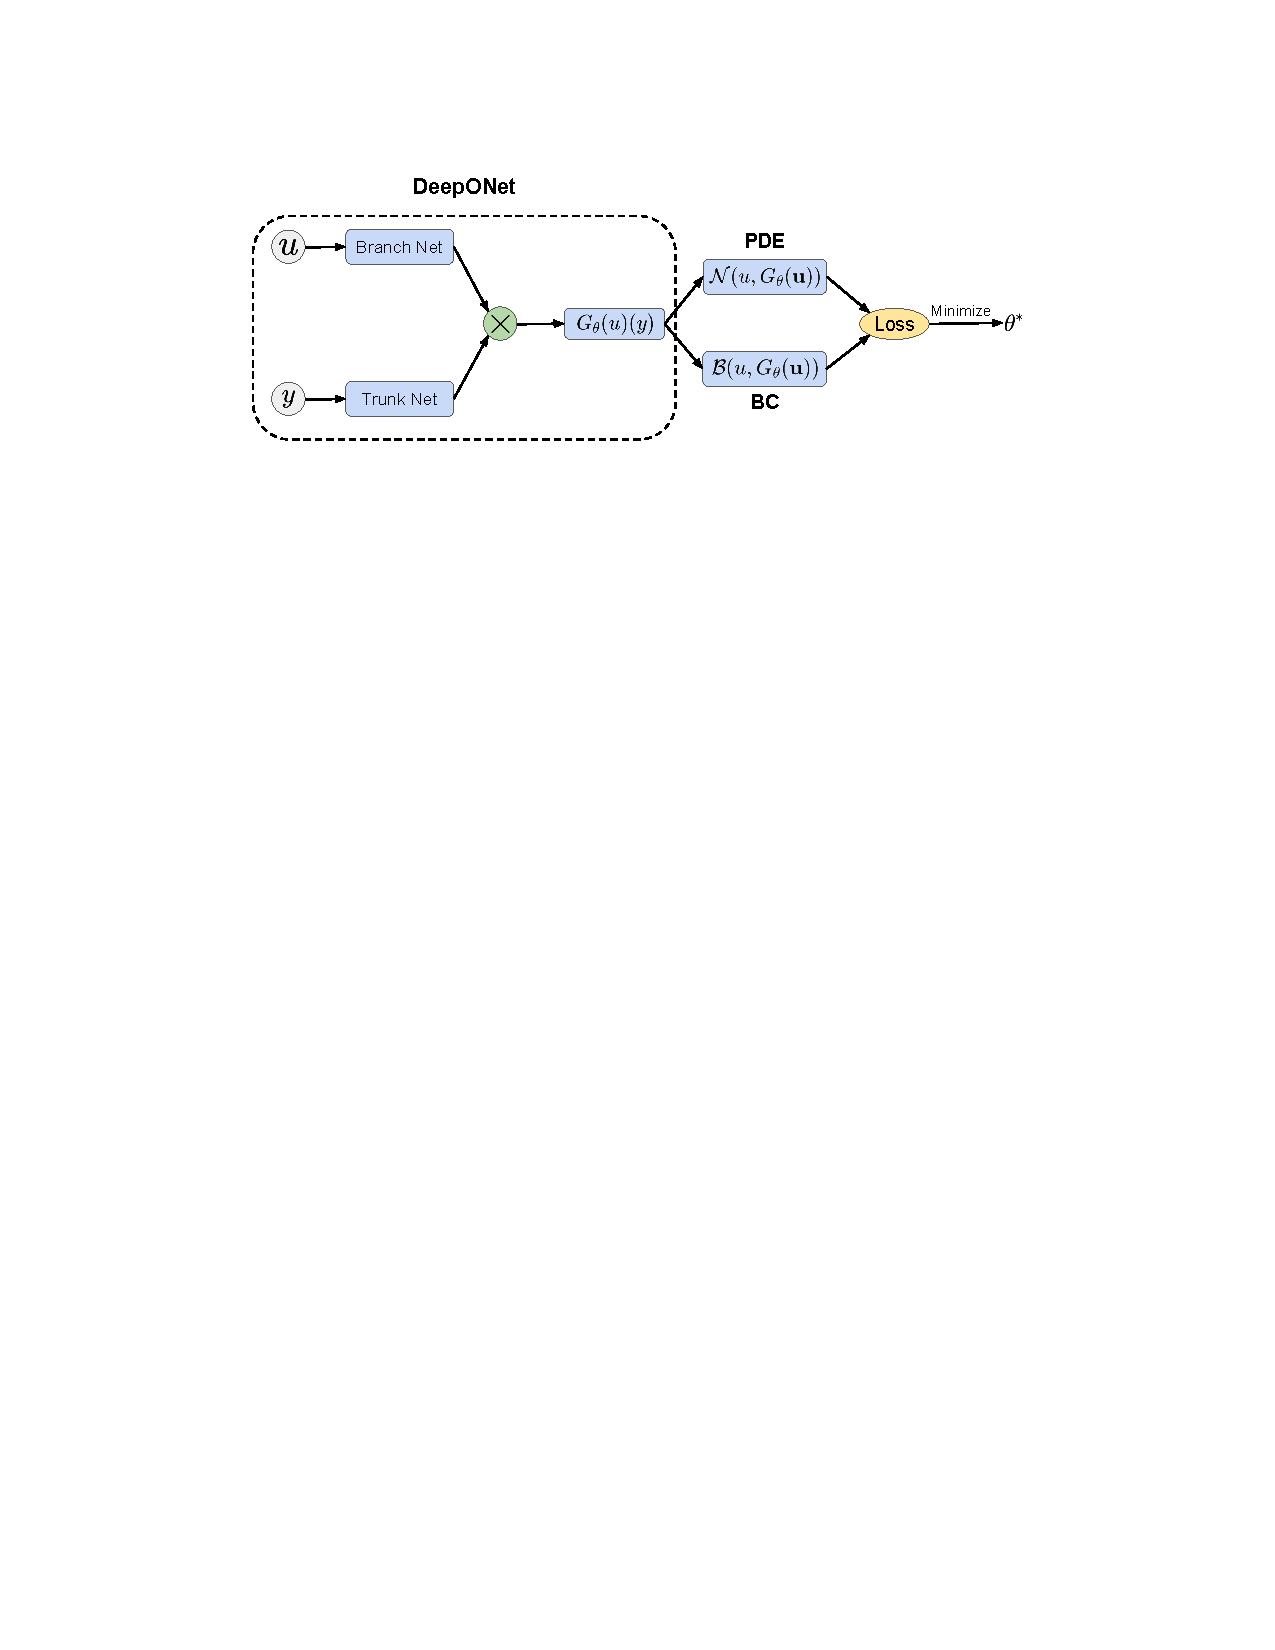
\includegraphics[width=1.1\textwidth]{../../../../../../1Research/Glotin/talks/DeepO_NTK}
\par\end{center}

{\tiny{[}Credit: Wang, Wang, Perdikaris; arXiv, 2021{]}}{\tiny\par}
\begin{itemize}
\item Train by \textcolor{magenta}{minimizing} the composite loss
\[
\mathcal{L}(\theta)=\mathcal{L}_{o}(\theta)+\mathcal{L}_{\phi}(\theta),
\]
 where 
\begin{itemize}
\item the \textcolor{magenta}{operator loss} is as above for deepOnet, or
using the IBC
\[
\mathcal{L}_{o}(\theta)=\frac{1}{NP}\sum_{i=1}^{N}\sum_{j=1}^{P}\left|\mathcal{B}\left(u^{(i)}(x_{j}^{(i)}),G_{\theta}(u^{(i)})(y_{j}^{(i)})\right)\right|^{2}
\]
\item the \textcolor{magenta}{physics loss} is computed using the operator
network approximate solution
\[
\mathcal{L}_{\phi}(\theta)=\frac{1}{NQ}\sum_{i=1}^{N}\sum_{j=1}^{Q}\left|\mathcal{O}\left(u^{(i)}(x_{j}^{(i)}),G_{\theta}(u^{(i)})(y_{j}^{(i)})\right)\right|^{2}
\]
\end{itemize}
\item This is \textcolor{magenta}{self-supervised}, and does not require
paired input-output observations!
\end{itemize}

\foilhead{$\;$}

\vfill{}

\begin{center}
{\Large\textbf{\textcolor{blue}{OTHER METHODS}}}{\Large\par}
\par\end{center}

\vfill{}


\foilhead{Differentiable Physics}

A potentially powerful \textcolor{magenta}{hybrid} approach is to
open up the black box of a traditional algorithm and tightly integrate
ML models within it. 
\begin{itemize}
\item This allows a more granular way of balancing the two paradigms; 
\begin{itemize}
\item \textcolor{magenta}{ML} can be inserted where we are unsure how to
solve a problem, or where the traditional workflow is computationally
expensive, and
\item \textcolor{magenta}{traditional} components can be kept where we require
robust and interpretable outputs. 
\end{itemize}
\item Often, the performance of the traditional workflow is improved whilst
the ML components are easier to train, are more interpretable, and
require less parameters and training data compared to a naive ML approach.
\item A general approach for doing so is to use concepts from the field
of \textcolor{magenta}{differentiable physics}
\begin{itemize}
\item many traditional scientific algorithms can be written as a composition
of basic and differentiable mathematical operations (such as matrix
multiplication, addition, subtraction, etc), and that 
\item modern \textcolor{magenta}{automatic differentiation} and differential
programming languages {[}Baydin et al., 2018{]} make it easy to track
and backpropagate the gradients of these outputs with respect to their
inputs. 
\item This unlocks the possibility of inserting and training gradient-based
ML components (such as neural networks) \textcolor{magenta}{within}
traditional workflows, whereas otherwise it may have been difficult
to do so.
\end{itemize}
\item A simple approach to start with is to re-implement a traditional workflow
inside a modern differentiable programming language, such as PyTorch,
TensorFlow or JAX. 
\item Once a traditional algorithm is implemented, its design can be altered
by treating certain parameters as \textcolor{magenta}{learnable},
or by inserting new learned components.
\end{itemize}

\foilhead{Neural ODEs}
\begin{center}
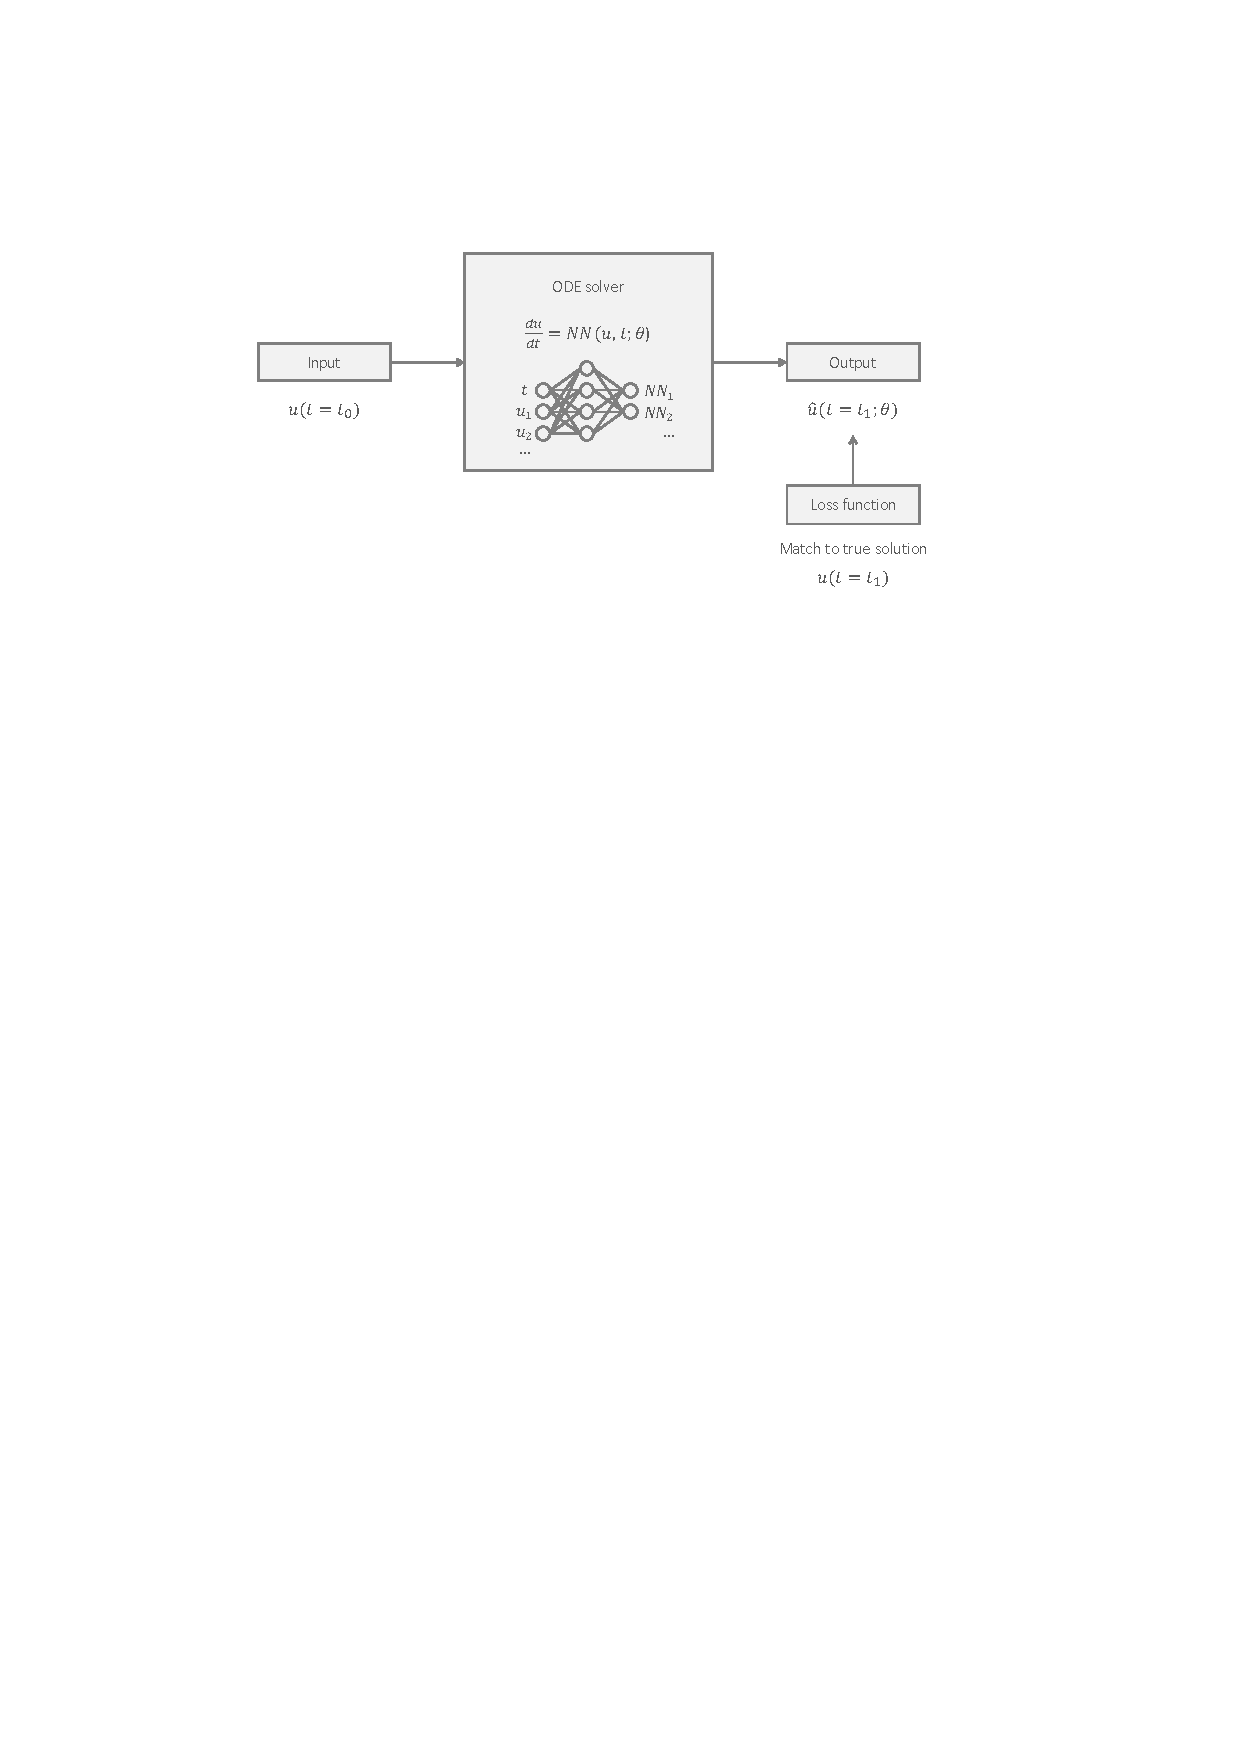
\includegraphics[width=0.8\textwidth]{graphics/neuralODE}
\par\end{center}

Schematic of a neural ordinary differential equation (ODE) {[}Moseley2022{]}. 
\begin{itemize}
\item The goal of a neural ODE is to learn the right-hand side term of an
unknown ODE.
\item A neural network $\mathrm{NN}(u,t;\theta)$ is used to represent this
term, which is trained by using many examples of the solution of the
ODE at two times, $u(t=t_{0})$ and $u(t=t_{1}).$ 
\item More specifically, a standard ODE solver is used to model the solution
of the ODE, $u(t=t_{1}),$ at time $t=t_{1}$ given the solution at
time $t=t_{0}$ and evaluations of the network where needed. 
\item Then, the network\textquoteright s free parameters, $\theta,$ are
updated by matching this estimated solution with the true solution
and differentiating through the entire ODE solver
\end{itemize}

\foilhead{Other Approaches}
\begin{itemize}
\item Recurrent NNs - see FIDL example
\item Material design (META) uses Graph NNs
\item GP and Ridge regression - used by Mendez
\item LSTM
\item Encoder-decoder
\item in fact the list is never-ending...
\item and now there is \textcolor{magenta}{generative} learning!
\end{itemize}

\foilhead{$\;$}

\vfill{}

\begin{center}
{\Large\textbf{\textcolor{blue}{GENERATIVE PHYSICS LEARNING}}}{\Large\par}
\par\end{center}

\vfill{}


\foilhead{GPT}
\begin{itemize}
\item GPT = Genrative Pre-trained Transformer
\item Theory:
\begin{itemize}
\item ingest huge volumes of data
\item ``fill in the gaps'' using Markov Chains on tokens
\end{itemize}
\item Applications
\begin{itemize}
\item NWP + Climatology (ClimaX by Microsoft) 
\item healthcare and drug-design (Alpha-Fold)
\item etc.
\end{itemize}
\item Quo Vadimus??? See \textcolor{blue}{Introductory and Ethics Lectures}
for more details.
\end{itemize}

\foilhead{$\;$}

\vfill{}

\begin{center}
{\Large\textbf{\textcolor{blue}{APPLICATIONS}}}{\Large\par}
\par\end{center}

\vfill{}


\foilhead{Applications of ML for (P)DEs}
\begin{itemize}
\item Literally, from ALL domains...
\item See next lecture.
\end{itemize}

\foilhead{Bibliography-Reviews}
\begin{thebibliography}{1}
\bibitem{key-23}S A Faroughi, N Pawar, C Fernandes, M. Raissi, S.
Das, N K Kalantari, S K Mahjour. Physics-Guided, Physics-Informed,
and Physics-Encoded Neural Networks in Scientific Computing. arXiv,
2023. \url{https://arxiv.org/pdf/2211.07377}

\bibitem{key-24}S. Cuomo, V. Schiano Di Cola, F. Giampaolo, G. Rozza,
M. Raissi, F. Piccialli. Scientific Machine Learning Through Physics--Informed
Neural Networks: Where we are and What\textquoteright s Next. \emph{Journal
of Scientific Computing} (2022) 92:88.

\bibitem{key-25}L Lu, P Jin, G Pang, Z Zhang, GE Karniadakis. Learning
nonlinear operators via DeepONet based on the universal approximation
theorem of operators. \emph{Nature Machine Intelligence} 3 (3), 218-229
(2021).

\bibitem{key-2}L. Lu, X. Meng, Z. Mao, G. Karniadakis. DeepXDE: A
Deep Learning Library for Solving Differential Equations. \emph{SIAM
Review,} 63, 1 (2021).

\bibitem{Darve} E. Darve, K. Xu. Physics constrained learning for
data-driven inverse modeling from sparse observations. \emph{J. of
Computational Physics}, 453. (2022).

\bibitem{Karnia}M. Raissi, P. Perdikaris, G. E Karniadakis. Physics-informed
neural networks: A deep learning framework for solving forward and
inverse problems involving nonlinear partial differential equations.
\emph{J. of Computational Physics}, 378, pp. 686-707, 2021.

\bibitem{Stuart}N. Kovachki, Z. Li, B. Liu, K. Bhattacharya, A. Stuart,
A. Anandkulmar. Neural Operator: Learning Maps Between Function Spaces
With Applications to PDEs. \emph{J. of Machine Learning Research }24
(2023).

\bibitem{Asch2016} M. Asch, M. Bocquet, M. Nodet. \emph{Data Assimilation:
Theory, Algorithms and Applications.} SIAM, 2016.

\bibitem{Asch2022}M. Asch. \emph{Digital Twins: from Model-Based
to Data-Driven.} SIAM, 2022.

\end{thebibliography}

\end{document}
